\documentclass{article}

\usepackage[utf8]{inputenc}
\usepackage[margin=2cm]{geometry}
\usepackage{multicol}
\usepackage{color}
\usepackage{float}
\usepackage{graphicx}
\usepackage{pdfpages}
\usepackage[style=authoryear-ibid]{biblatex}
\usepackage[hidelinks]{hyperref}

\graphicspath{{images/navigation/}{images/app/}{images/overview/}{images/machinelearning/}}

\addbibresource{references.bib}

\def\labelitemi{--}

\title{Software Design Study Report}
\author{A-Team\\Matthias Casula, Lewis Dawson, Joe Groocock, Chris Lane, Tyler Stopforth}

\begin{document}
\maketitle

%\tableofcontents

\begin{abstract}
  Cars are ubiquitous in our modern lifestyles, unfortunately, the software systems in them do not keep up with other computing systems that we use. In this report, we aim to show how we tackled the problems and areas for improvement that we found in current car systems. Five areas of a modern car's feature set were focused on weekly, these being; the dashboard, media, navigation, safety and an accompanying smartphone app.
\end{abstract}

% \begin{multicols}{2}

\section*{Introduction}
For years car companies have invested relatively little into their car's information systems and technological abilities. Inbuilt satellite navigation systems are often hard to use and update, and are generally counter-intuitive. Since these companies are slow to adopt new technologies, even features that would have been possible many many years ago have not been widely adopted yet. For example, we still use the physical dials in the instrument cluster that we have used for years.

We have created an attractive and modern solution for digital technology in a car that we hope to see in future modern cars in production. In Section~\ref{sec:system-design} we will give explain the technical elements of our system design that can be found ranging from navigation to safety features. In Section~\ref{sec:nav} we will go into detail on the design process of our navigation system. In Section~\ref{sec:app} we will go into detail on the design process of our accompanying smartphone app.

Some further documentation is linked to in Section~\ref{sec:appendix}, which aims to assist the understanding of this report. At the end of this appendix, we have included slide decks outlining the entire design of the system, annotated to reflect our designs going forward.

\section{Overall system design}\label{sec:system-design}
\subsection{General}\label{ssec:system-design-general}
Our system is built of many separate components which together work seamlessly, these are the centre console, the instrument cluster, in-door screens, and a dashboard-mounted navigation screen. There is also, of course, the smartphone application that will be installed on user mobile devices which perfectly compliments the system.

The instrument cluster is an LCD display located behind the steering wheel. This displays the usual car instrument information such as speed and fuel level. It is also customisable with widgets to display relevant information for example weather forecast for local and destined locations, currently playing media information and general vehicle health and status. 

The door-mounted screens are dumb 5-inch touchscreen displays located in the arm rest of each rear door. These serve the purpose of allowing back seated passengers to control media playback by queueing and ordering songs of their choice either to the whole car or to their own headphones/speakers.

The navigation screen is a 6 inch display located above the dashboard and it displays the street map and directions while driver is using navigation. We kept this display separate from the centre console to reduce the distance the driver has to look whilst driving and using navigation.

The instrument cluster, rear back door screens and navigation screen are connected to the centre console via a network of serial cables. Data is sent between these devices and it consists of information for the console to process and what to display on the devices screens.

This centre console is the central computing unit for the car which runs on an Android based operating system. The backing system for this, and all dumb interfaces in the car, uses a feature originating in modern Android phones which provide a dual-system architecture. Initially, both systems are flashed with the same image; as updates are installed, the other system image is written to then booted into as the new primary system after a successful install. This leaves the other system as a complete bootable image in the case of corruption or other fatal disasters rendering the updated system unusable. This alternating behaviour of `ping-pong' between the two partitions is used for every update to ensure a more reliable and stable system.

Finally there is an auxiliary system separate from the centre console which processes all sensor data collected from the myriad of sensors and cameras all around the interior and exterior of the car, and hosts and runs the safety systems. Separation of these two computers is deliberate to keep computation of critical safety systems unhindered from the general user-facing computation of the central computing unit such as navigation and media consumption.

\subsection{Algorithms}\label{ssec:algorithms}
To perform the route calculation for the navigation system we are using Bi-directional A* search to create routes from a start position to a destination. This will with include custom heuristics based on the users history and various other relevant sources. This is explained in more detail in Section~\ref{sssec:nav-tech-routing}~[\nameref{sssec:nav-tech-routing}].

We take advantage of K-means clustering at the start of a convoy routing to group together convoy members before they begin their journey. This will guide drivers to a central location based on each member's location in the group. This is discussed in more detail in Section~\ref{sssec:nav-tech-kmeans}~[\nameref{sssec:nav-tech-kmeans}].

As a safety feature we detect if drivers are distracted by tracking their face pose. We have a camera for tracking the drivers face in the driver-side pillar directed at the seat, and we process this feed using ASM landmarks. This reliably gives us information on where the driver is looking, according to the conclusion~\cite{head-pose} made comparing ASM with other head pose detection methods. With this information we can make an informed decision and ultimately conclude if the driver is distracted and act accordingly.

We also keep a brief history of head poses exhibited by the driver, to analyse as part of tiredness detection. If the drivers eyes are closing for long periods of time or their head is lowering frequently, we trigger tiredness alleviation responses such as turning on air conditioning and suggesting that they are re-routed to a service station.

\begin{itemize}
  \item Learning algorithm --- user preferences, Contextually Aware Routing etc
    % FIND A LEARNING ALGORITHM
  \item Safety Detection algorithms
    \begin{itemize}
      \item Tesla radar system?
      \item Recognising bikes --- trained from training images which are bikes with riders
        % This is if we are detecting bikes using this method of detecting bikes (we mentioned using the 360 degree vision from the cameras for seeing bikes)
    \end{itemize}
  \item Something for tiredness detection
\end{itemize}

\subsection{Storage}\label{ssec:storage} % Chris
Our design has three places that data will be stored, some data being temporary and some persistent. We will store information in the cloud, in the car's local SSD storage and on the smartphones belonging to the users of the app.

The cloud will be used for the majority of storage, it is where persistent data will be synchronised to from the phone app and car. Storage for most data such as user profiles will be kept in an encrypted Oracle database. The cloud will store user profiles that contain details such as saved routes, privileges, seat preferences, dashboard layout, contacts and driver stats. The cloud will also store details about convoy groups, containing data on members, member locations, group messages, routes etc. Since the cloud hosts the API used by the car and app, other miscellaneous data will also be stored here such as software updates.

The car's internal SSD storage will be used for fast reading and writing of synchronised files and cached data primarily. Data queried from the cloud will be cached to grant a more seamless experience even when the car is not connected to the internet. Examples of cached data from the cloud include favourite routes, dashboard layout and seat positions. Since the centre console system is built around the Android platform, we have been able to easily allow certain apps from the Play Store. One example of an app that we would allow on the system is Spotify, for music playback. The Spotify app will be able to store all of its settings, cached data and offline playlists in the car's internal storage as well. Local music files synchronised from a home network will be stored in the car's internal storage.

The dashboard cameras will also record their video to the internal storage of the car, this will be limited to a default percentage of the drive capacity (the storage SSD can be upgraded) and recordings will overwrite old footage in order to reuse the assigned storage space. The basic version of the system will likely have at least 120GB of SSD storage, however, this could easily be upgraded by swapping out the drive from the glove box.

The system files are stored on a separate disk elsewhere in the car with the redundant backup system (see Section~\ref{ssec:system-design-general}~[\nameref{ssec:system-design-general}]) to allow for hot-swapping of the storage drive. This system allows the storage drive to be upgraded, replaced or swapped at any time without affecting the running system.

The accompanying car smartphone app does not require much storage at all since it must be connected to the internet or car to make any changes. Data from the cloud, car and app will be cached so that it may still be accessible for short connectivity outages.

\subsection{Data Structures}\label{ssec:data-structures} % Chris
In the system that we have designed, we require a few different data structures in order make our system efficient and easy to work with.

For our navigation algorithm, we decided to model the street map as a graph. Road junctions, route starting point and route destination are all represented as nodes in the graph, with roads being the edges that connect the nodes of the graph. This graph structure is most appropriate for us to use in our bidirectional A* search algorithm.

Routes will be kept in a JSON format with a JSON object containing two lists, one list containing nodes IDs of a route and the other containing the edge IDs. List items will be in chronological order for the route. The system is able to present the route on-screen by reading the lists to build the section of the street map graph that represents the route. This JSON format also allows for sections of the route to be updated easily by swapping out and adding nodes and edges. Another benefit of this format is that it is easy to implement the transferring of these routes from the app to the car.

The customisable dashboard layout will also be stored in a JSON format with widgets stored in a list object and more general details in a separate object. Widget objects in the list contain information about their relative position, size and styling in the dashboard.

User profile data such as username, route preferences etc.\ will all be kept in an encrypted Oracle database in the cloud, this will allow for us to have granular control over what information we receive when requesting user information.

An SQLite database will exist in the local storage of the car, this database will contain details of local music files that are also stored in the car's local storage. Music files that have been added to the car will have their song, album and artist names looked up and stored in the database. The SQLite database provides access to song details to the centre console and car app.

The smartphone app for the car system will use the same data structure for maps as the car uses. Cache data from the cloud and car will be stored in an SQLite database.

\subsection{User Accounts}\label{ssec:user-accounts} % Matt
Something that we found is lacking across intelligent car systems in the market is the use of portable user profiles. By this we mean profiles that can be used across several cars, applying user settings and preferences where applicable.
These user profiles are shared from car to car by syncing user information files from the cloud. This is only done when the user has logged into the car and authenticated themselves with the cloud.
\subsubsection{Storage and transport}
The method we found most suitable for doing this works by storing the data relative to each user profile in an local SQLite database. Information is then served directly to the car or mobile phone when a user logs in on the device. This is only if the login is verified by the cloud. The data is cached on the phone and car, as applicable, to allow access to user profile information even when internet access is limited or not available.
\subsubsection{Cardinality of accounts, vehicles and shared data}
Each user will have one account that will be able to contain multiple car profiles. Car profiles can share generic information, such as preferences regarding routing, music, favourite temperatures, speed dial contacts, etcetera if the user specifies so. Information specific to the car make and model, such as steering rack height, seat adjustments, wing mirror adjustments shall stay bonded to each car profile.
\begin{figure}[H]
  \centering
  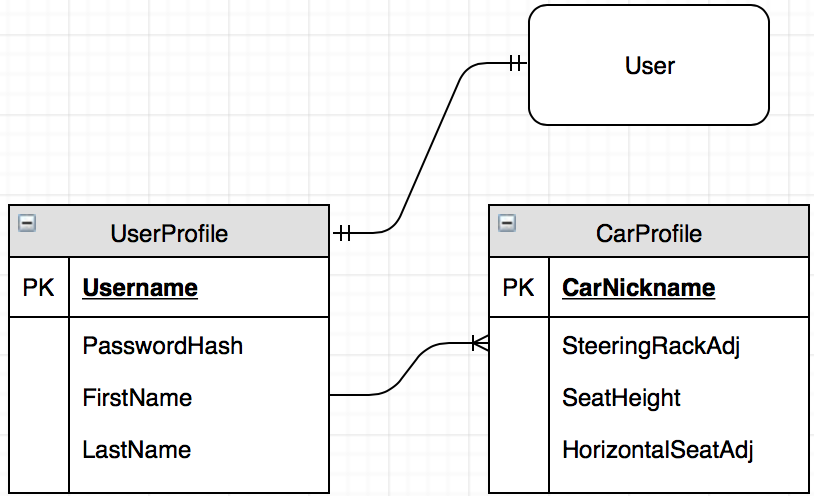
\includegraphics[scale=0.7]{profile-cardinality}
  \caption{Visualisation of cardinality of user profiles}\label{cardinality}
\end{figure}

\subsection{Communications \& Data Flows}\label{ssec:communications-data} %Tyler
Within our system, we have communications between the Mobile App, the Car and our Cloud, with links to external APIs.

\subsubsection{Communication between devices and cloud}\label{sssec:car-cloud}
The car and mobile app communicate with the cloud mainly to synchronise information. The device sends hashes and timestamps of their files to the server, which compares them with the latest versions. The files which are different are sent back to the devices for synchronisation.

Since the car and the mobile app can both change user profile settings, there will be continuous syncs when user settings or preferences are changed. This is so the user can change their settings away from their car with their phone, and have them set up automatically the next time they enter their car.

The car and mobile app both share the same routes and search destinations that have been entered on each device. Again this is synced through the cloud using the method explained above.

The software within our car has standard API requests that will always have a response from our cloud, we decided that the cloud would have a general API service, which would provide a link to the external APIs that we use. This is so we can provide the best API for a given location, and there is no unnecessary traffic going through our cloud. Also if external APIs are unavailable unexpectedly, we can always just update the cloud to provide a new link to a different external API\@. These services are mentioned in more detail in Section~\ref{sssec:devices-APIs}~[\nameref{sssec:devices-APIs}].

During navigation in convoys, the car's location is sent to the cloud and the associated group member's locations are pulled down from the cloud. This is so the location of other group members can be regularly updated on the navigation display. Other information such as group messages or navigation reroutes are also communicated between group members and the cloud.

All the system updates for the car's software will be downloaded from the cloud. These files will be verified using MD5/SHA1 hashes and comparing them to the hash provided by the cloud server. This is to ensure they are not corrupted or tampered with.

The cloud will always be listening for real-time event data. This is the kind of events that would be happening live, such as if someone is breaking into your car or for some reason the car alarm has just gone off. Once in the cloud, this information would be passed straight to the car owners phone via the app to alert them.

\subsubsection{Communication between car and phone}\label{sssec:car-phone}
Communications between the car and the phone consist of initial connection, instructions and data transfer. Establishing a connection is done by pairing the phone to the car by means of NFC, this will authenticate the phone with the car for communications over Bluetooth and Wi-Fi. Authentication can also be achieved by typical manual methods such as typing in a password. There will also be the standard Bluetooth communication between the phone and the car such as sharing contacts and taking calls.

Many features of the app communicate with the car, these features are described in Section~\ref{ssec:app-tech}~[\nameref{ssec:app-tech}]

\subsubsection{Communication between devices and external APIs}\label{sssec:devices-APIs}
Many sections of our system gather a lot of information from external APIs. This information ranges from data required for navigation to getting the latest weather forecasts.

While using navigation, the car will automatically get the latest information on roadworks, current traffic conditions and information on public transport. This information will be based on the location of the car and is used to add displays to the map. For example showing roadworks in locations where road work is occurring.

Our dashboard can contain widgets to display simple information like weather which would be pulled down from the cloud and updated regularly.

\subsection{Information Security}\label{ssec:information-security} % Joe
A major focus for any internet connected technology is security, and with our car systems it is no different- the last thing a customer would want is to have their car stolen by it being driven into the distance by a remote thief. We employ a model of `encryption everywhere' to ensure maximum data security, paired with very strong authentication to prevent unauthorised access or control. Security is a primary focus in every aspect of the car system, the following non-exhaustive list are some of our main focuses

\subsubsection{Data Communication}
Every connection that is made in our ecosystem leverages the flexibility and security of TLS for both encryption and authentication. TLS provides a strong suite of ciphers cross-compatible with any device. Industry standard hardening techniques are employed at both client and server end to ensure the strongest connection possible such as only using strong mutually-agreed cipher suites and key exchanges.

This widespread usage of full transport encryption is viable due to the hardware-accelerated AES-NI and similar instruction sets built into most modern CPUs by manufacturers like Intel, AMD and ARM* (dependent on model and chip manufacturer). Without hardware support, encryption would be very expensive in terms of computation for every device: servers, cars and most importantly mobile devices such as smartphones and embedded devices.

Performing AES or similar encryption purely in software is very slow and consumes a significant amount of CPU cycles and battery power resulting in a poor experience thus making encryption on lower power and mobile devices not at all feasible.

Another advantage of using TLS is `Perfect Forward Secrecy' of data when the appropriate key-exchange protocol is used such as a Diffie-Hellman based exchange method. This provides the guarantee that any data that is intercepted in transport by a 3rd party cannot decrypt the data with a previously apprehended pre-shared key or certificate as the short-lived session token has been lost.

\subsubsection{Data Storage \& Encryption}
Wherever sensitive account or user data is stored, regardless of device is is advised that storage encryption is used at some level to provide some protection against data loss or theft. Most preferably a TPM or other hardware cryptographic device is present in the system to perform disk or filesystem level encryption. Many devices such as laptop \& desktop computers and many modern smartphones provide such functionality covering a wide majority of use cases. Otherwise an alternative storage method can be used where all stored or cached data is encapsulated in a single container or image and encrypted with a simple AES pass using a key stored in user account on a cloud server so it can always be accessed.

\subsubsection{User Authentication}
We leverage the implicit authentication flow from TLS backed by per-user certificates (specification defined at \url{https://tools.ietf.org/html/rfc5246#appendix-F.1.1}) which is a security advantage to the cloud provider  as it is more secure authentication method than using a password and presents a cleaner user experience as it requires no input from the user whereas a password would do.

Everywhere a persistent login is used, it is replaced with a client certificate authorised to access the account without a password. The primary use of these certificates is the automatic authorization of the mobile app on smartphones and embedded devices with the cloud servers and the car. The certificate must be present for communications with a car and is preferred for authenticating with cloud servers as it provides significantly better security than a password and requires less interaction from the user.

For each additional device that a user adds to their account, a unique certificate is generated and stored on the device therefore allowing each user device to be tracked individually, linking the device to the specific user.

Further discussed in Section~\ref{ssec:app-security}~[\nameref{ssec:app-security}] are additional security features used specifically within the mobile application for extra convenience and protection.

\subsubsection{Server and Car Authentication}
Similarly to user authentication with certificates, each car system has an inbuilt signed certificate from the car manufacturer to prove it's authenticity. The matching private key for the certificate is installed in a hardware keystore within the car computer to improve it's robustness against attacks and is communicated with over a standard bus built into the car computer system.

Unlike the mobile app, the car must always use it's certificate when communicating with any external service and can only communicate over the encrypted and authenticated HTTPS protocol. This is to ensure no future attacks are developed by exploiting the availability of unencrypted communications.
The car system will only handshake successfully with services that it recognises immediately or those which have been signed by a recognised authority, as any HTTPS connection should.
Any system in the car that is not directly tied to critical or sensitive services may continue to use a standard CA (certificate authority) list; it is only internal services used directly by the car that requires the manufacturer-trusted CA store.

The cloud security situation is very similar. Each server is provisioned with a certificate/key pair, signed by the cloud provider and governing body, which are used to handshake every connection to the car and mobile app.
It is important that all endpoints communicating with these services ensure they check the validity and authenticity of the TLS certificates to prevent unwanted data leakage or MITM (man-in-the-middle) attacks where some critical authentication or identifying information could potentially be stolen. Any attacker posing as a rogue cloud server could forge certificates and assuming the client (whether that be an app, web client etc) doesn't verify it is signed by the correct authorities then the attacker can read all data passed to it unencrypted, as it was originally sent.

\subsubsection{Device Certificate Revocation}
Certificates can be revoked individually, on a per-device basis; this allows a user to instantaneously prevent any unauthorised access to the car in the case a phone/laptop is lost or stolen.

A user can revoke a certificate from their account at any time via the web portal or by calling the manufacturer's helpline, both of which are critical high-availability services as the security of vehicle control is paramount. Upon revocation, repeated push calls are made to every device on the account, including the car, to advise of the updated access  control. This is important as while many services are always authenticated through the cloud services like `remote access' of the vehicle (where revocation would immediately apply), some processes such as local unlocking via NFC or accessing the in-car computer only authenticate locally for speed and would have to wait for the revocation update to be received. \textit{It should be very clearly noted that car ignition requires sufficient cloud authentication so the car cannot be started with any revoked certificate, ever.}

\subsubsection{Wi-Fi Hotspot}
Every car is required to provide a 802.11ac Wi-Fi (or faster) access point to the passengers within and nearby the car to provide internet access via the in-car mobile data connection, as well as access to internal services in the car such as media controls and data transfer.

Adhering to modern standards, in-car Wi-Fi only uses the most recent WPA2 specification for encrypting wireless traffic. This standard enforces the use of AES which is hardware backed in most processors and is the industry standard for general data encryption. Two options are presented to users for authentication:
\begin{itemize}
  \item `Pre-Shared Key (PSK)' Mode: This is the most commonly used method of Wi-Fi authentication using a single static key that which is entered on every device that connects to the network. The key can be customised in the `Settings' app in the car
  \item `Extensible Authentication Protocol (EAP)' Mode: Business and education establishment networks are the primary users for this authentication method however it provides a much more secure approach to authenticating users against the network. It works with a username \& password combination unique to that user which is validated externally of the wireless network; in this case it is validated on the cloud servers using the login of the user account for the person logging in.
\end{itemize}

\noindent It is advised that most people use EAP for Wi-Fi connectivity as it provides better security benefits, but it can also be desirable to run an WPA2-PSK network alongside the primary EAP for guest users who don't have an account or devices that do not support WPA2-EAP authentication.

\subsubsection{Two Factor Authentication}
To promote good security habits, users are advised to enable `2 Factor Authentication' on their accounts via the standard method specified by~\cite{rfc6238}. 2FA is a security tool which requires a second factor of authentication in the form of a 6 digit number, generated based on a seed provided by the cloud server which can either be generated from within any `authenticator' app or from within the phone app if the user is logged in.

When a login attempt is generated, a notification is sent to any device that the user is logged in on requesting to authenticate the new login and accepting will fulfil the request after logging in, bypassing the need to enter the code on the new device.

\subsection{Interaction Design}\label{ssec:interaction-design} % Matt + is this done?
The interaction designs used on our product's interfaces were designed loosely based on designs from industry leading companies but tailored to integrate our ideas and implement some recurrent suggestions found throughout our research, which has seen over 100 responses. Our product requires three main interactive interfaces for users to effectively communicate with the in-car system:

\subsubsection{Centre console}\label{sssec:centre-console}
This is a 10-inch touchscreen located in the middle section of the dashboard. Its purpose is that of displaying most of the information that flows through the car that may be of interest to the user and for the user to interact with it. For instance, destination input for the navigation system, joining and managing convoys, customising the instrument cluster, querying the system for detailed engine data and many more interactions will be performed on this device.

We found that in the recent years the integration of touch screens on dashboards has become a recurrent trend amongst major manufacturers and believe that it is an essential feature for the cars of the future due to how visible, versatile and aesthetically pleasing they are.

\subsubsection{Mobile app}\label{sssec:mobile-app}
As usage of mobile apps is constantly increasing, more and more industry leading companies are adopting this as a new mean of interaction with their automobiles. We firmly believe that this will become and essential feature to all cars within a few year and therefore have designed and prototyped one. More detail can be found in Section~\ref{sec:app}~[\nameref{sec:app}].

\subsubsection{Device on rear doors}\label{sssec:device-rear-doors}
Each of the rear door cards will be fitted with a 5-inch touchscreen device that enables passengers in the rear of the car to search and add songs to the cars' shared music queue from different streaming services or a local library.

\subsection{Aesthetics/Graphical Design}\label{ssec:aesthetics}
% Matt
% User Interfaces of the above devices
An effort was made to follow current styling standards used in industry to give the user a familiar experience, therefore flat designs were used where possible. Also characterising our design are large icons and avoidance of large swathes of text.

\subsubsection{Instrument cluster screen}\label{sssec:cluster-screen}
A screen will be replacing the usual instrument cluster behind the steering wheel. This will display information relative to speed, engine revolutions, fuel levels as it has been doing for the past decades but with the difference of being fully customisable in layout, content and colour. These features will result in improved user experience for individuals with poor vision and colour blindness since font sizes and colour schemes can be altered easily in the settings. More generally, as suggested by our questionnaire research, the majority of users will enjoy having the ability to select what they will see behind the steering wheel themselves. The LCD panel in question will not be a touch screen since access would be restricted by the wheel and the customisation will be managed on the centre console screen instead.

\subsubsection{Centre console}\label{sssec:centre-console-aestethics}
The design of this interface is simple and intuitive, its main menu is made up of large square buttons that are labelled with text that have an adjustable size. Since this is intended to be the main point of contact between the user and the cars' infotainment system, different types of information are displayed on it ranging from navigation menus to engine management information. While opening new activities on similar devices is usually simple, switching between them isn't always as intuitive and that is why our interface has a virtual button in the top left corner labelled with the name of the previous activity so that the user can easily switch to the previous one. The backgrounds are static to prevent causing unnecessary distractions, however, the colour scheme is fully customisable by the user and is carried through to all of the interfaces in the car.

\subsubsection{App}\label{sssec:app-aestethics}
The design choices for our mobile app are detailed in Section~\ref{ssec:app-design}~[\nameref{ssec:app-design}].
\subsubsection{Rear side door}\label{sssec:rear-door-device-aestethics}
This interface has limited functionality, its purpose is that of enabling the passengers in the rear to contribute to the queue of songs being played on the car. Given this, its appearance is designed to be minimalist with a button per available library/streaming service.

%%%%%%%%%%%%%%
%
%	NAV
%
%%%%%%%%%%%%%%
\section{Feature 1: Navigation}\label{sec:nav}

\subsection{Research}\label{ssec:nav-research}
As part of the brainstorming process, we investigated current technology to see how the current navigation systems were perceived by various people. The first part of this research takes the form of a questionnaire we created to gather opinions on both current technology as well as some of our own ideas. From this, we confirmed our beliefs that most people use their phone as their navigation assistant; and are generally happy with current methods of controlling a SatNav, being touch screen and voice control.

We also gained some insight into some design decisions we should take, with a majority of survey participants being interested in seeing friends travelling with them; speed cameras; traffic; and road obstacles such as roadworks, accidents and breakdowns, on the map --- while there was less interest in tracking emergency and breakdown recovery vehicles. There is also a greater interest in having various destination suggestions available to the driver. The survey indicated to us that some features are already being executed well in existing systems and most people find the directions given by their SatNav to be quite clear.
% Link to survey responses?

We also performed some research to find out exactly what kind of features are currently offered by SatNav systems. As part of this research, we discovered that a lot of our brainstorming ideas are already in active development by some companies. A lot of these concepts are being produced by Google into usable products already: if you search for a location on Google Maps, there is an option to send the location to the Maps app on your phone; your movements are analysed by Google to determine favourite places and routes. Google uses the data collected from your location and search history to better provide suggestions for future searches. They also infer useful information based on frequent and popularly visited destinations to generate smartphone notifications suggesting users where to visit.  

During this research, however, we could not find any recent implementation nor professional research into our ideas for the concept of `convoy driving'. The closest concept to this we could find was the `Garmin Tracker' which seems to have very limited functionality for tracking a person who owns a Garmin branded SatNav, for purposes such as knowing when a family member should arrive home. It also appears that this feature is only included in a limited subset of the Garmin models, which seem to have been discontinued. \cite{garmin-tracker}~mentions the existence of this tracker, stating ``this could be useful if you are in a big group and you have more than one car travelling to the same destination'', but does not elaborate further, and we cannot find documentation from Garmin as to whether this is the exact use of this tracker.

\subsection{Brainstorming}\label{ssec:nav-brainstorming} % Matt
% Should we include our initial ideas document?
In the first stage of our brainstorming we created a Google document which allowed us to collaboratively write down any initial ideas we could come up with. By discussing them within our group, new ideas kept being generated and even different variations of the ideas we already had. In order to keep the design space as open as possible  during this stage, all ideas were noted down and considered, no matter how far-fetched. Following this initial stage, and an iteration of research, we went through the document and filtered through it as a group, moving concepts that we wanted to bring forwards into our refined design. During the second stage of brainstorming, we created a new document, containing only the best of our ideas to expand and research them in more depth.

An aid we found very useful was personas: a list of made-up personalities with realistic interests, jobs and attributes. During the brainstorming each of us tried to empathise with each of the different personas and think about their habits, things they may enjoy, their mental states throughout different times of the day and from there, consider their needs and features in a navigation system they may want and enjoy and why.
% The personas are mentioned here, do we introduce them somewhere? Should it be in a research section or expanded upon here? -Lewis
Some of the ideas that came from our brainstorm are: 
\begin{itemize}
	\item Convoy tracking using K-Means clustering
    \item Public transport integration (including park and ride suggestions)
    \item Route scheduling via either the mobile app or in-car interfaces.
\end{itemize}

\subsection{Technical Background}\label{ssec:nav-tech}
\subsubsection{Routing algorithm}\label{sssec:nav-tech-routing}
The routing algorithm we use is bidirectional A* search, performing a typical A* search from the start node to the destination, and another from the destination to the start node, in parallel. The aim is to produce a complete path by using the central intersection of the two searches from either end. The heuristic used for this search will incorporate:
\begin{itemize}
  \item Learnt user habits \& preferences, applying lower weight to road types preferred by the driver such as if they frequently divert through smaller roads, and applying a higher weight to road types that tend to be avoided by the driver as well as preference of `fastest route', `most direct route' or `shortest distance'
  \item Roadwork and traffic information, gained from the APIs, which will apply a higher weight to roads based on their traffic levels
  \item Traffic balancing using mass telemetry from other nearby vehicles, splitting traffic evenly across the possible routes to ease congestion on a larger scale. This option particularly is heavily weighted as to reliably keep traffic load split as evenly as possible
\end{itemize}
To ensure the route continues being optimal, the system polls the APIs every five minutes for updates to traffic conditions and roadworks. After this data has updated the graph, the search is re-run, with the start node being ahead of the current position in order to account for the latency in running the search. The search also re-runs when the driver leaves the current route, to make sure they are still travelling efficiently.

\subsubsection{Machine learning}\label{sssec:nav-tech-machinelearning}
In order to suggest the optimal route for a specific user, the navigation system will make use of a Recommender System, which is a piece of software that uses a Machine Learning algorithm, more specifically a Classification Tree (see Figure~\ref{decision-tree}) in order to guess a rating for a small set of routes based upon user habits. 
The 3 routes with the highest ratings will be shown to the user as a result of their search. Each tree represents a user profile created using the user’s preferences, extrapolated from the features of the routes they normally take, including how scenic a route is, type of roads (main or back roads), likelihood of heavy traffic at the current time and whether the driver is currently tired or not. 
All the possible features are placed in a binary vector, where each row corresponds to either of the features listed above. The rows of each vector that correspond to a specific feature of a route are marked with a one, while the rest is marked with a zero. Content-Based filtering is being used throughout this approach as we only use data relevant to the current user and do not compare data from different users as collaborative or hybrid filtering would do. By taking into account the current level of tiredness of the user we are not only producing a context-aware Recommender System but a Risk-Aware one that aims to recommend the safest option at all times. For example if the drivers are tired and the route results include motorway and non motorway options then the recommender would likely assign the latter a higher score.

The choice of machine learning was inspired by research, the papers we found most helpful were [Reference the 2 papers i asked lewis to add]. The decision was then reinforced by the observations that decision trees of such depth require very little computational time and power and are easier to implement that other methods, such as neural networks, ensemble and matrix factorisation-based methods.

\begin{figure}[H]
  \centering
  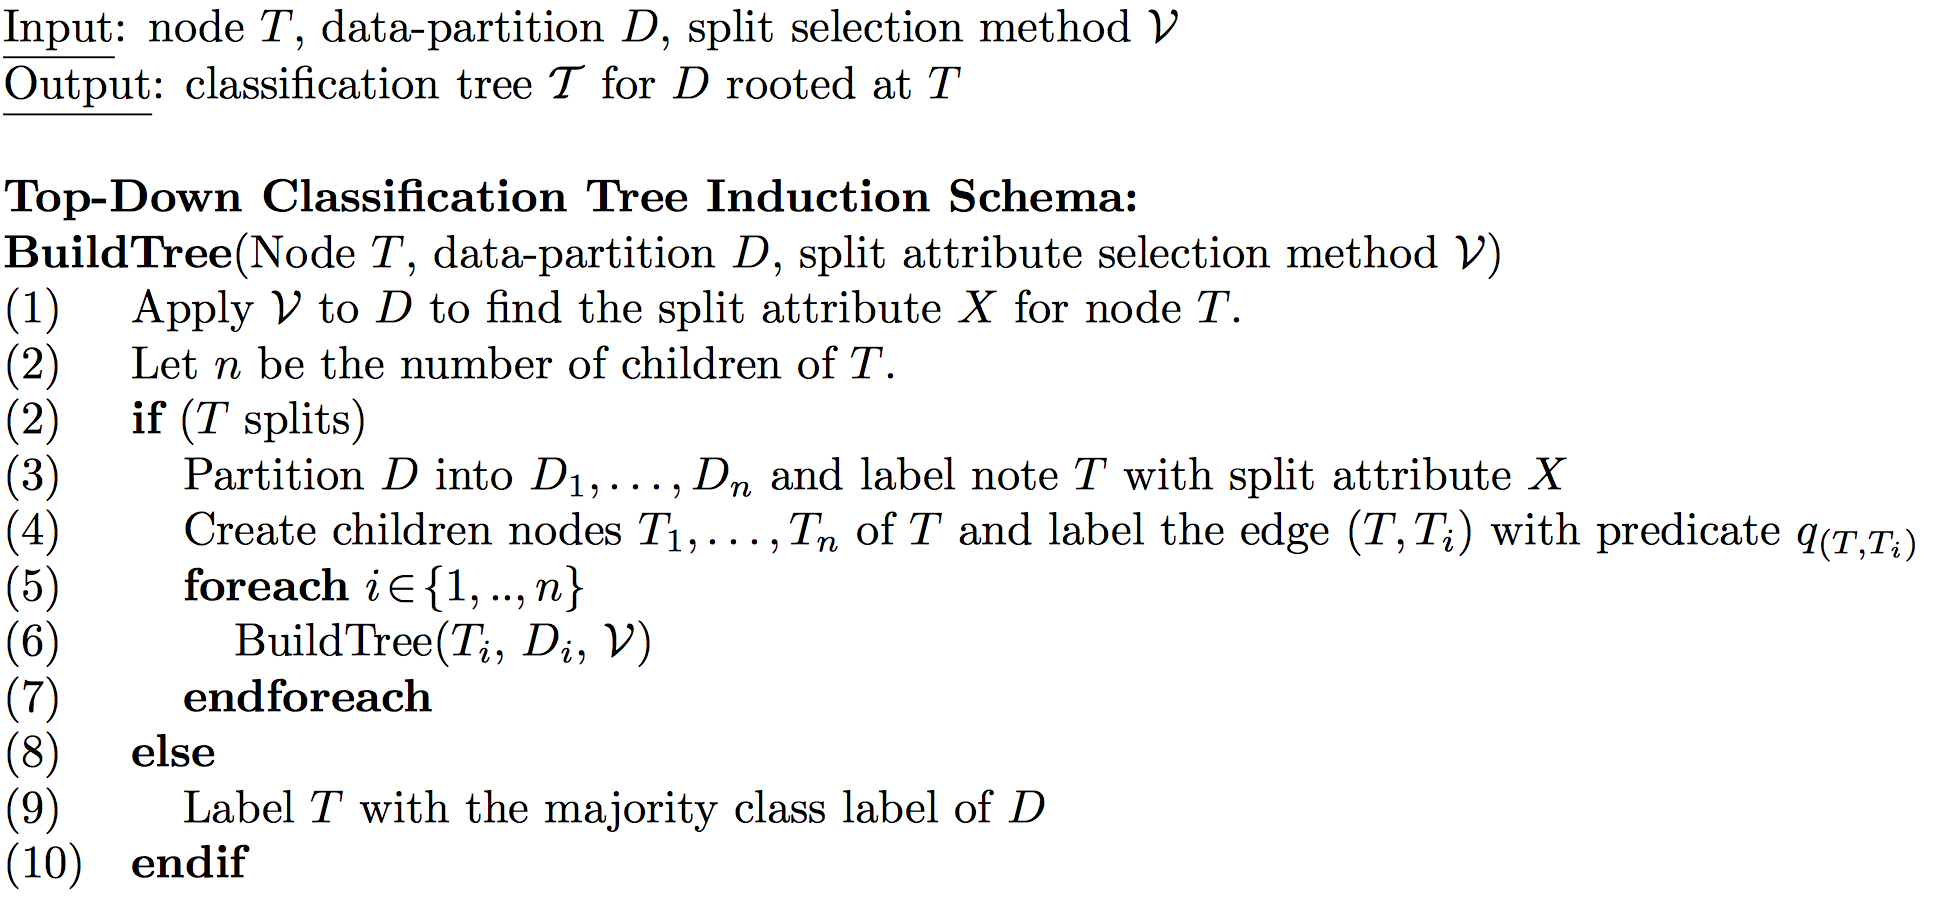
\includegraphics[width=0.9\textwidth]{decision-tree}
  \caption{Classification tree induction schema}\label{decision-tree}
\end{figure}

\subsubsection{K-means clustering}\label{sssec:nav-tech-kmeans}
One of the problems we encountered while designing the convoy feature was how to handle situations where a group is starting its journey separated, and quite widely spread. From our brainstorming sessions, we decided to implement k-means clustering as a method for grouping the members of a convoy together. As described in Figure~\ref{nav-kmeans}, any members of a convoy who wish to group together as quickly as possible to travel together on the main shared route will be grouped together through clustering. A number, $k$, (explained later) of ``means'' are randomly placed on the graph, and then two steps are repeated until the optimal positions for the means are found --- determined by them not moving from the previous iteration.

The first step is to create the clusters (step 2 of Figure~\ref{nav-kmeans}), associating each member of the convoy to their nearest mean. The second step moves each mean to the centroid of their corresponding cluster. When convergence is reached, the means are moved to the closest suitable waypoint on the underlying map, and each cluster of convoy members is routed to this waypoint in their cluster. When the entire group is starting within the same city, assuming the destination lies outside the city, this should be sufficient; however, as the convoy gets more spread, this algorithm becomes less efficient, since members may be travelling very far individually before they reach their cluster waypoint. The solution here is to iterate the algorithm multiple times, with the start nodes of each iteration being the cluster waypoints generated by the previous iteration, reducing $k$.

There are some further issues with this algorithm that need to be addressed. Firstly, a good value for $k$ should be chosen. This value represents how many clusters are created by the algorithm, and therefore the average number of people (or groups, if this is a later iteration) to be grouped together by a given iteration can also be determined from $k$. Therefore, $k$ should be chosen based on how many people should be grouped up during one iteration; the standard default will aim to group together 3
%
% Requires a choice and justification
%
people (or groups of people) per iteration, meaning by default that $k=\frac{number\ of\ input\ nodes}{3}$. This may need to be changed or adapted based on the context, and can also be chosen by the convoy leader, where they can specify how many should group up, per iteration; the leader can also specify to not use clustering, allowing each driver to decide how they reach the destination.

The second issue arises when this algorithm would introduce a large inconvenience for certain members. In Figure~\ref{nav-kmeans}, it can be seen that the topmost blue member of the convoy starts out close to the destination, but the algorithm forces them to travel in a different direction. When the algorithm detects that the clustering route is significantly longer than a standard individual route, it presents an option to that member to accept the longer route, allowing them to group up with the others as quickly as possible; join directly into the full shared route, so they can still travel with the other members, but won't join up with them as quickly; or ignore the clustering, and follow an individual route, so they can reach the destination as quickly as possible while sacrificing the ability to travel in the main group.

\begin{figure}[H]
  \centering
  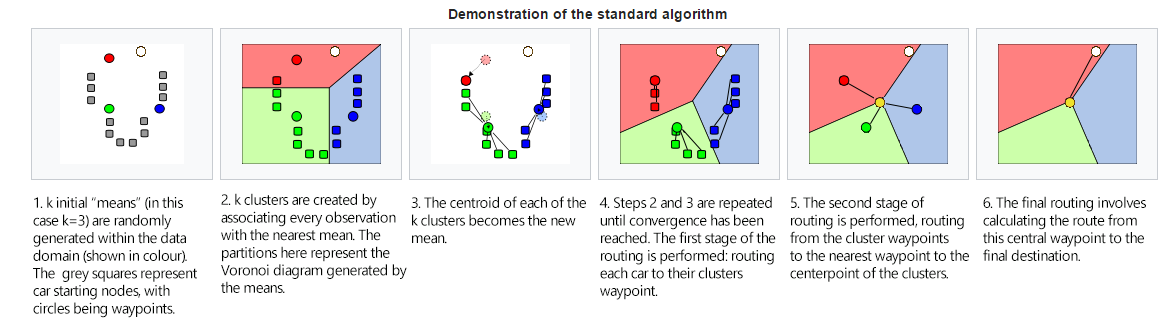
\includegraphics[scale=0.55]{kmeanscluster}
  \caption{Demonstration of K-means convoy clustering.}\label{nav-kmeans}
\end{figure}

\subsubsection{Public Transport}
A lot of people use public transport in their daily commute and so it seems logical to provide public transport information when the system thinks/knows that the user is heading to some sort of public transport hub. For example, if someone lives in a town outside London, they might drive to the train station to get to London every week day. The navigation system knows from the knowledge from the machine learning algorithm that the driver is going to drive to the train station and so it can display train times for the estimated time of arrival. The machine learning will also have learnt if there is a specific time that the driver usually arrives at the station and so can inform the driver whether they are likely to be late or not.

Public transport information is pulled from an API chosen by the cloud to give the best information for the destination.

\subsection{Convoy}\label{ssec:nav-convoy} % Chris
Convoys are a feature in our system, designed to allow a party to all route to the same destination, tracking members and having functionality for scheduled stops, rerouting and group calls. From the navigation menu, the user can select to either set up or join a convoy. The user that chooses to set up a convoy is given a six-digit code that they can then share via social media or any other way. Users that choose to join the convoy must enter the six digit code they were given by the convoy creator. The convoy creator is able to set the route destination, any stop off points and optionally give the convoy a name.

Once a convoy is set up, members of the convoy are able to see the shared route and coloured icons for members on the map. In the case that convoy members are starting their journey from different places, members will be grouped, with groups having different routes to a point of convergence. Like the normal navigation mode in our system, the route for an individual can be adjusted to re-route them back to the convoy in the case that they go the wrong way. Another feature of the convoy system is that it provides the ability to make group VoIP calls so that users can communicate hands-free, this is done using peer-to-peer technology over the car's internet connection (provided it has one).

Users may want to use convoys despite being far apart from each other, in this case, users may not be likely to arrive at similar times and so routes are individually calculated on each car's system and uploaded to the cloud. Each user follows their own route and can see the expected time of arrival for other members in a sidebar. Should two routes converge at any point, members will be moved onto a shared route when they reach that point, making meeting up more likely and reducing the number of routes to be stored in the cloud.

A convoy member can leave the convoy at any time, however, there are points at which the system will prompt them to leave the convoy. The first occasion for a prompt is when the current driver of the car changes, the new driver might be wanting to travel to somewhere else. The driver can, of course, cancel the prompt, this is useful for a situation where for example people share the responsibility of the driving for a long journey. Another time that a prompt to leave a convoy may occur is in the event that all convoy members have arrived at the destination, at this point, there will typically be no further use for the convoy. The final situation for a prompt to leave a convoy is if the car is inactive for 24 hours, users typically will not be resuming a group journey after such a long time.

Convoy data is collected and distributed to all convoy members from the cloud. The cars will download routes via the cloud API and send GPS location updates to the cloud every few seconds, these location updates will then be pinged to all other convoy members to keep the location of cars synchronised on all screens. Once the cloud receives a new location for a member, it immediately deletes the old, redundant location.

Limited functionality of the convoys feature is available through the app. Users with the app are able to set up or join a convoy, this data is synchronised to the cloud and then used by the car.

There are of course limitations to this feature. Convoys require an internet connection to update member locations. If any member fails to update their location, their icon will stay in place and fade away until a connection is regained and the location is updated once again.

\subsection{Design choices \& Argumentation}\label{ssec:nav-design}
\subsubsection{General Design}\label{sssec:nav-design-general}
For a lot of features in our navigation section, we have utilised QOC as a method of deciding how to implement them. We have also used our survey responses as guidance for certain features.

We have employed a scoring system in the QOC in order to rank the options, which uses the importance levels of the criteria to determine how the options compare to each other.

\begin{figure}[H]
  \centering
  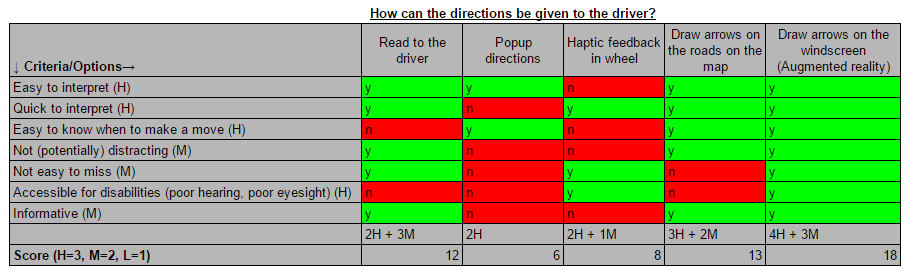
\includegraphics[width=\linewidth]{qoc-nav-instruction}
  \caption{QOC discussing how to direct the driver}\label{qoc-instructions}
\end{figure}

Figure~\ref{qoc-instructions} asks how directions can be given to the driver. As can be seen, an augmented reality approach appears to be a strongly decisive victor among these options, however, we had already discussed the ideas of augmented reality and head up display during the dashboard section of the design process, where we dismissed pursuing augmented reality for various reasons. For example, experiments conducted by~\cite{augmented-reality} conclude that ``the driver's attention to the road and traffic is likely to be compromised'' when HUD information is shown on the windshield. After some internal discussions we also feel that: it would be difficult to ensure it works in bright daylight while also working during night time; it would likely be expensive to implement and maintain, due to the high computational requirements as well as the cost of replacing projector bulbs; it may be difficult to reliably ensure the image lines up correctly to the drivers perspective, due to differences in head height or position; but we do not have substantial evidence supporting these claims.

As a result of dismissing the use of augmented reality for our final designs, the two currently popular methods of direction, delivery become the top choices from the QOC, and sticking with these choices seems to be a good idea since most of our questionnaire responders felt their SatNav devices were sufficiently clear already.

\begin{figure}[H]
  \centering
  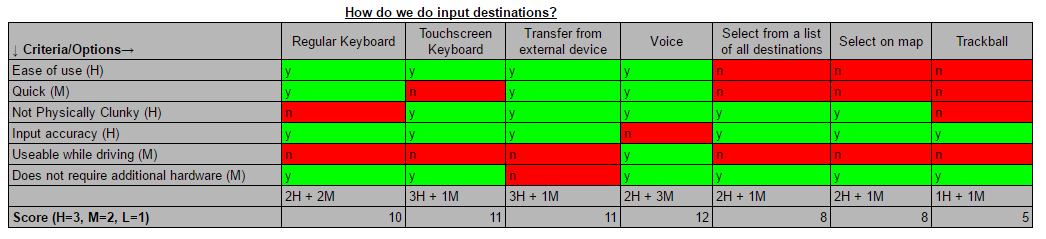
\includegraphics[width=\linewidth]{qoc-nav-input}
  \caption{QOC discussing how to input a destination}\label{qoc-input}
\end{figure}

Figure~\ref{qoc-input} asks how the driver should be able to input destinations to their SatNav. As expected, the current standard forms of input score the most highly, being voice and touchscreen keyboard, along with the ability to transfer from external devices. We also considered having a physical keyboard connected to the SatNav device, which also scored highly, but we decided that having a usable keyboard like this would be far too clunky to include.

Our final design features the ability to use all three of these input methods, allowing users to control the destination using the voice assistant
%
% We need to mention the existence of this elsewhere. (mentioned on trello)
%
in the car; a touchscreen keyboard which is displayed on the centre console; or sent to the car via the phone app, which is explained further in Section~\ref{sssec:car-cloud}~[\nameref{sssec:car-cloud}].

\begin{figure}[H]
  \centering
  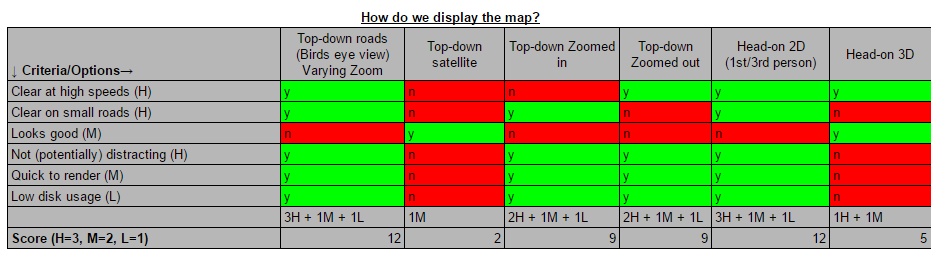
\includegraphics[width=\linewidth]{qoc-nav-map}
  \caption{QOC discussing how to display the map}\label{qoc-map}
\end{figure}
Figure~\ref{qoc-map} asks how the map can be displayed on the navigation screen. We considered designs such as top-down view with satellite picture, which looks nice but does not fulfil the other criteria. We also considered fixed-zoom top-down designs, but being a fixed zoom level would make it unclear in certain situations, which is solved by having varying zoom. This QOC determined that the currently popular designs are the most suitable: top down with varying zoom, and head-on display with flat buildings; so our final design allows the user to choose between these options.

\begin{figure}[H]
  \centering
  \fbox{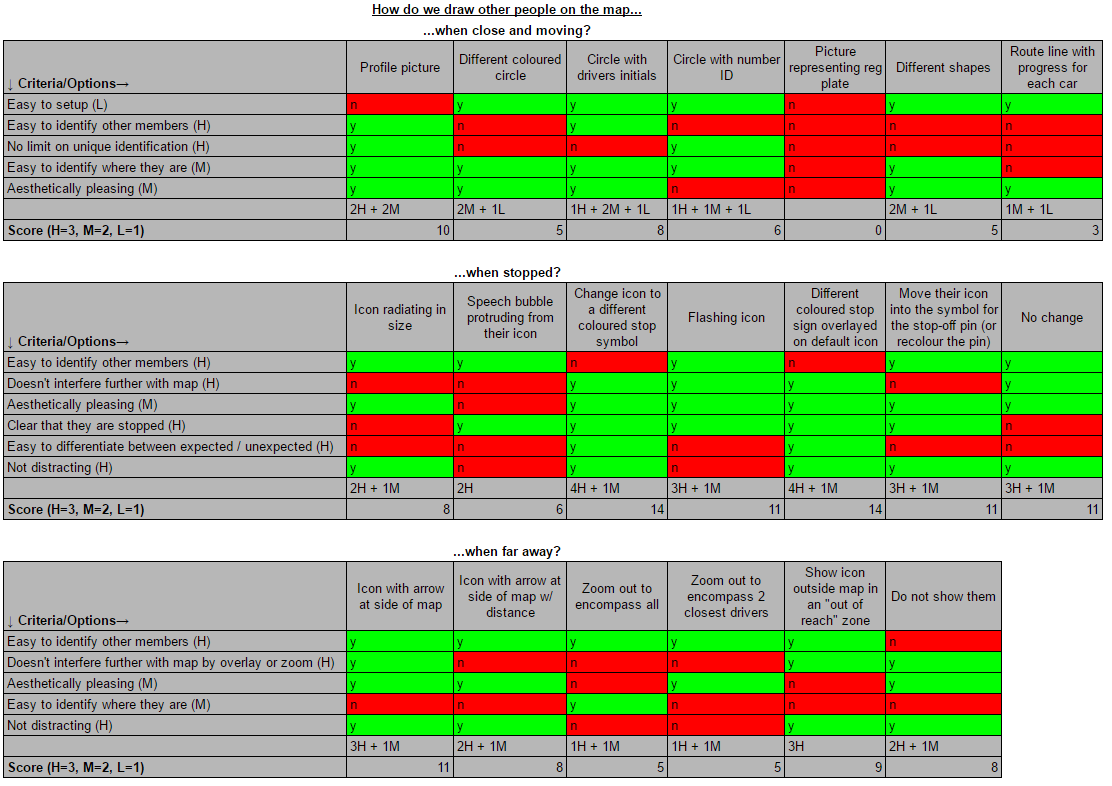
\includegraphics[width=\linewidth]{qoc-convoy}}
  \caption{QOC discussing how to display others in a convoy group}\label{qoc-convoy}
\end{figure}

Figure~\ref{qoc-convoy} asks how to represent other drivers in a convoy group on the map. We wanted the representation to distinguish between drivers who are moving and those who have stopped - and further, those who have made unexpected/unplanned stops - while also providing a suitable representation for if they are far away. We didn't have much to dispute with these QOC results, and all of the highest scoring options were taken through to the final design. As a mitigation for the profile picture being not easy to set up, we allow the user to sync their profile picture with social media, or to just use their initials. To allow further customisation, however, users may choose to have a basic coloured circle as their representation, since this may be desired especially in smaller groups.

\subsubsection{Algorithm Justifications}\label{sssec:nav-design-alg}
We used QOC as well as experimentation to determine which routing algorithm to use for navigation.

\begin{figure}[H]
  \centering
  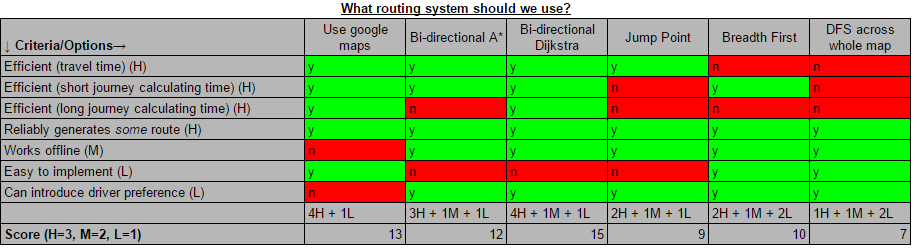
\includegraphics[width=\linewidth]{qoc-nav-routing}
  \caption{QOC discussing search algorithms to be used for navigation}\label{qoc-nav-routing}
\end{figure}

Figure~\ref{qoc-nav-routing} discusses the different approaches to routing that we found during research. The best option according to our scoring system here is to use Google maps, since we could give start and end locations to a Google maps API to ensure efficiency in both calculation time and route. This was, however, an early consideration in our design process, and we realised that there were some large limitations to using this approach: we could not adapt the underlying algorithm and heuristic to suit our needs, meaning we could not introduce the preferences of the driver into the generated route; we would be limited in design space, especially with the convoys, since it may be difficult correctly synchronising features like waypoints, as well as the generated route, across the convoy; we also wanted to ensure that the routing could be performed offline, since Internet connectivity is not something that can be guaranteed.

Bi-directional A* is therefore the algorithm we decided to use. We have access to the heuristic which allows us to introduce driver preferences and convoy waypoints; it works offline, as long as an offline map is stored; and it will still generate an efficient route, though it may be less so than if generated by Google maps.\\

We did not perform much research into clustering algorithms; we recalled k-means clustering from a previous University module and it worked well to do what we needed it for. Since this forms only a relatively small part of the overall system, and should only need to be used once per convoy route, there was very little to be gained from using a different algorithm for this.

We researched various machine learning algorithms to find some algorithms relating to the learning of user preferences. The first that we found, as described in Section~\ref{sssec:nav-tech-machinelearning}~[\nameref{sssec:nav-tech-machinelearning}], fulfilled our requirements for this, meaning that other algorithms would provide negligible benefit over this algorithm.
%
% Machine learning!
%

\subsection{Prototypes \& user testing}\label{ssec:nav-prototypes-testing}

\subsubsection{Lo-Fi Prototypes}
\begin{figure}[H]
  \centering
  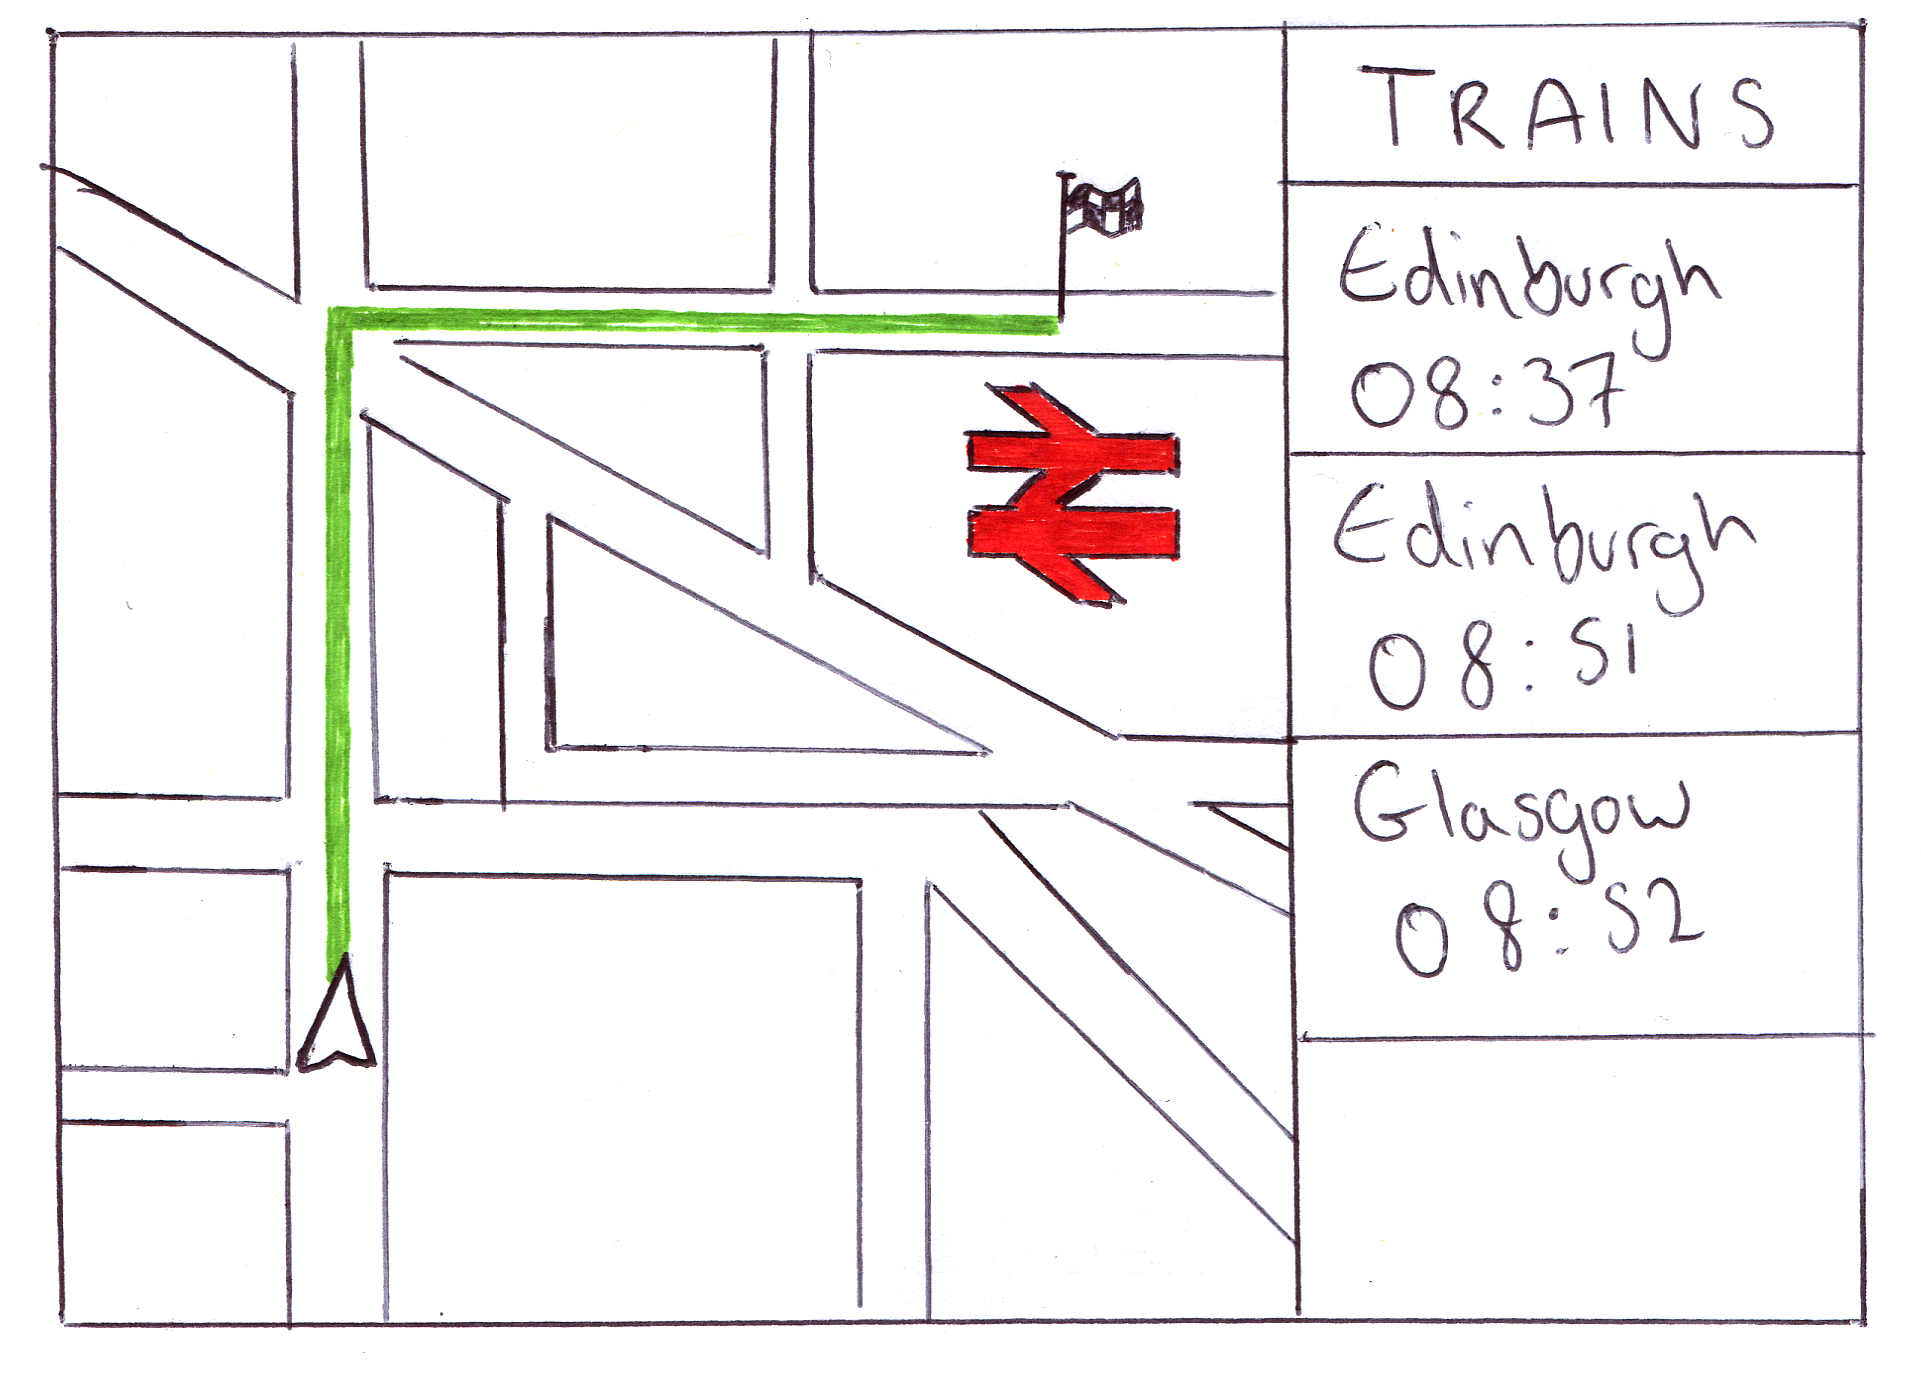
\includegraphics[scale=0.5]{train-widget}
  \caption{Lo-fi design for how public transport information could be integrated into navigation}\label{train-widget}
\end{figure}

It was clear to us that public transport would be a valuable feature in our final design, so we created a design to see how the feature would look. Figure~\ref{train-widget} shows a route with destination set to a train station. The next trains leaving the station within $\pm$15 minutes of the estimated arrival time are shown on a menu to the right of the map, as provided by the public transport API data.
\begin{figure}[H]
  \centering
  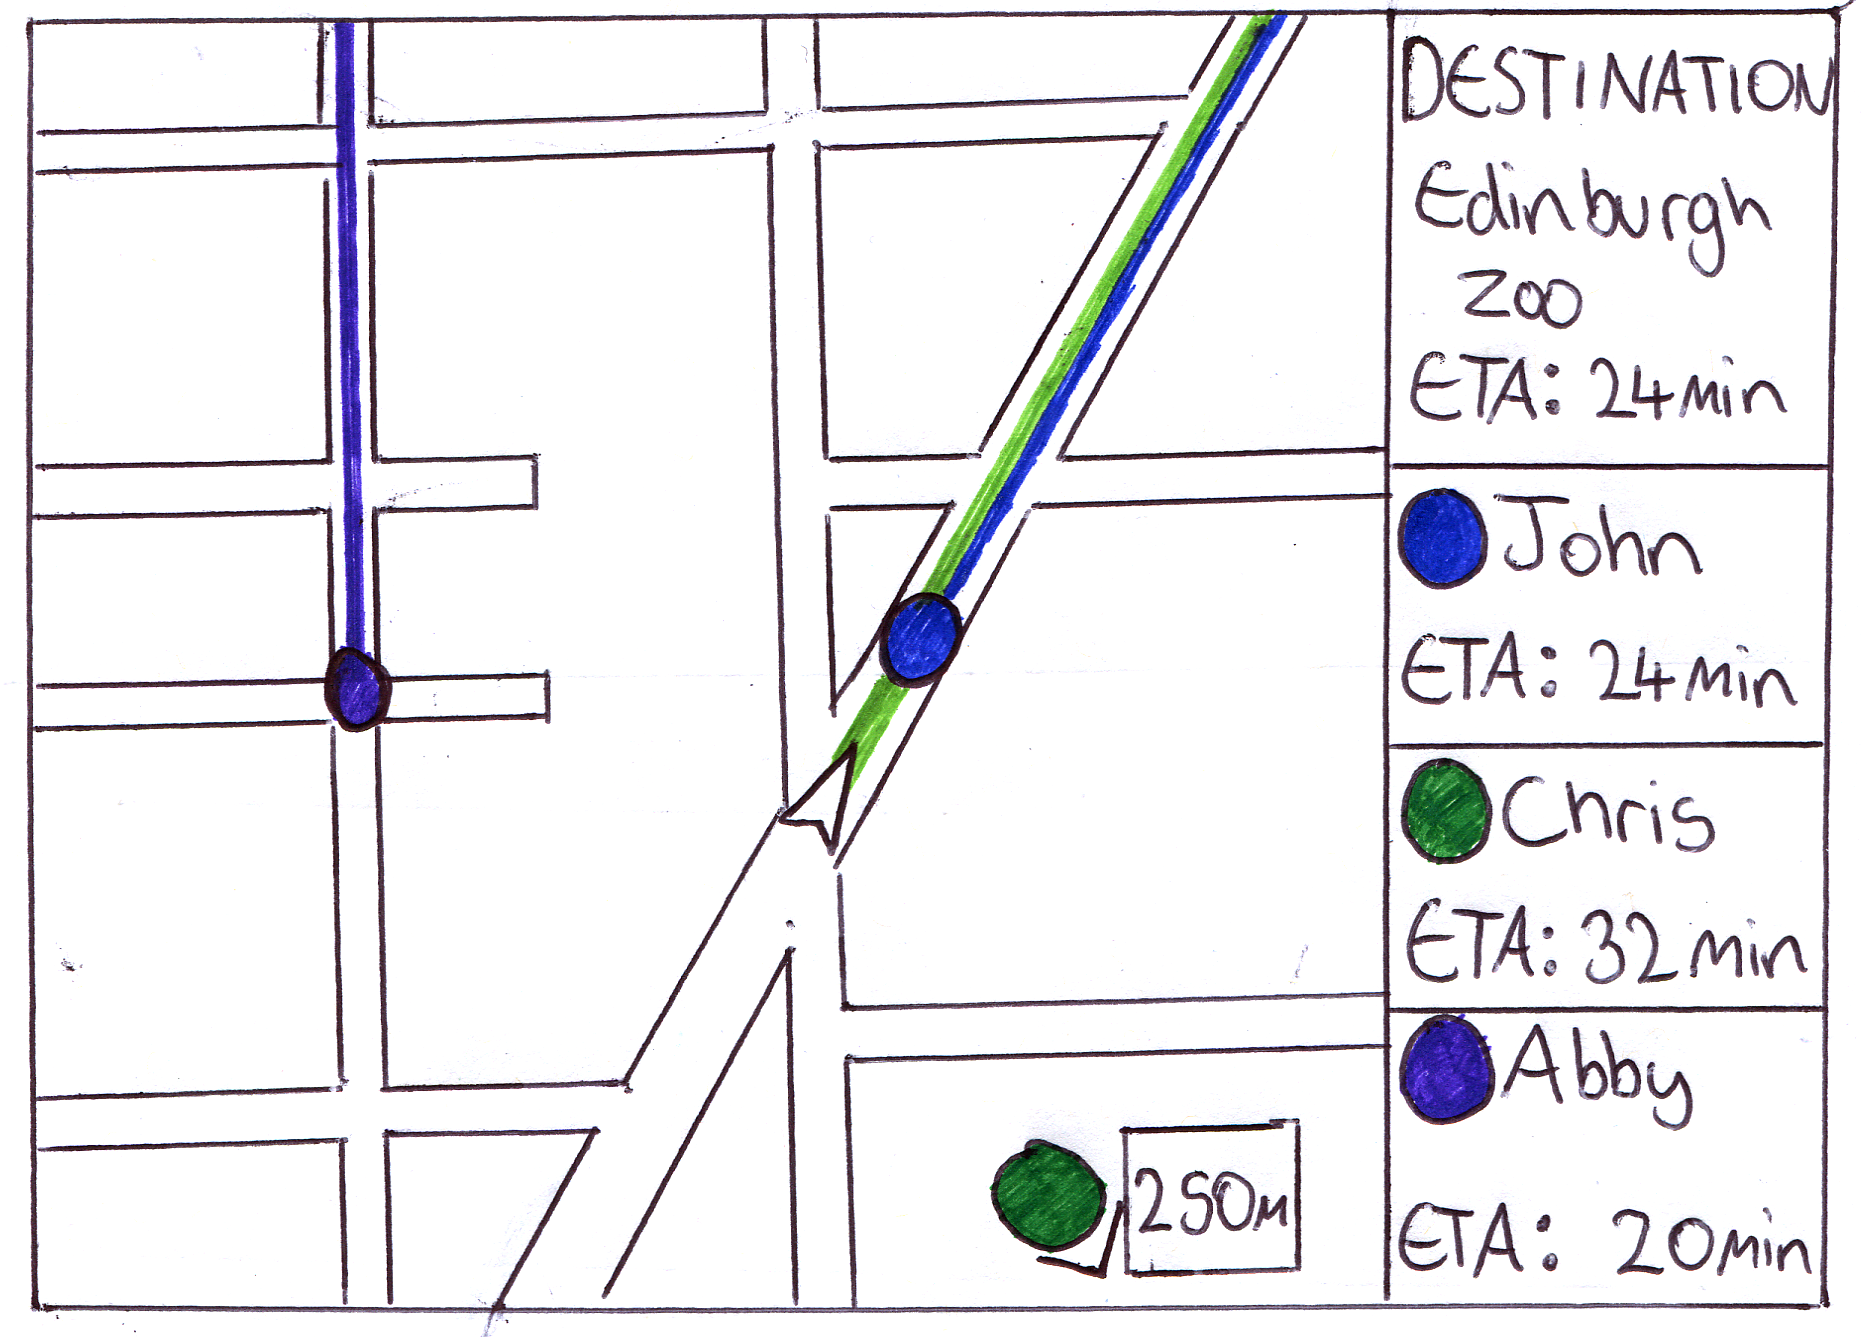
\includegraphics[scale=0.5]{convoy-lofi}
  \caption{Lo-Fi design for travelling different routes in a convoy}\label{convoy-lofi}
\end{figure}

We had a lot of ideas surrounding the convoy functionality, so we created a Lo-Fi design to see how some of our ideas might look. Figure~\ref{convoy-lofi} presents a convoy with four drivers, investigating how certain situations would be displayed. Here, we see that the white car (representing the driver of the current car) and the blue car are following the same route, with purple following their own route; and each route being displayed slightly differently. The green car is too far away to be displayed on the map, so is shown at the edge with an arrow.

\subsubsection{Hi-Fi Prototypes}

\begin{figure}[H]
  \centering
  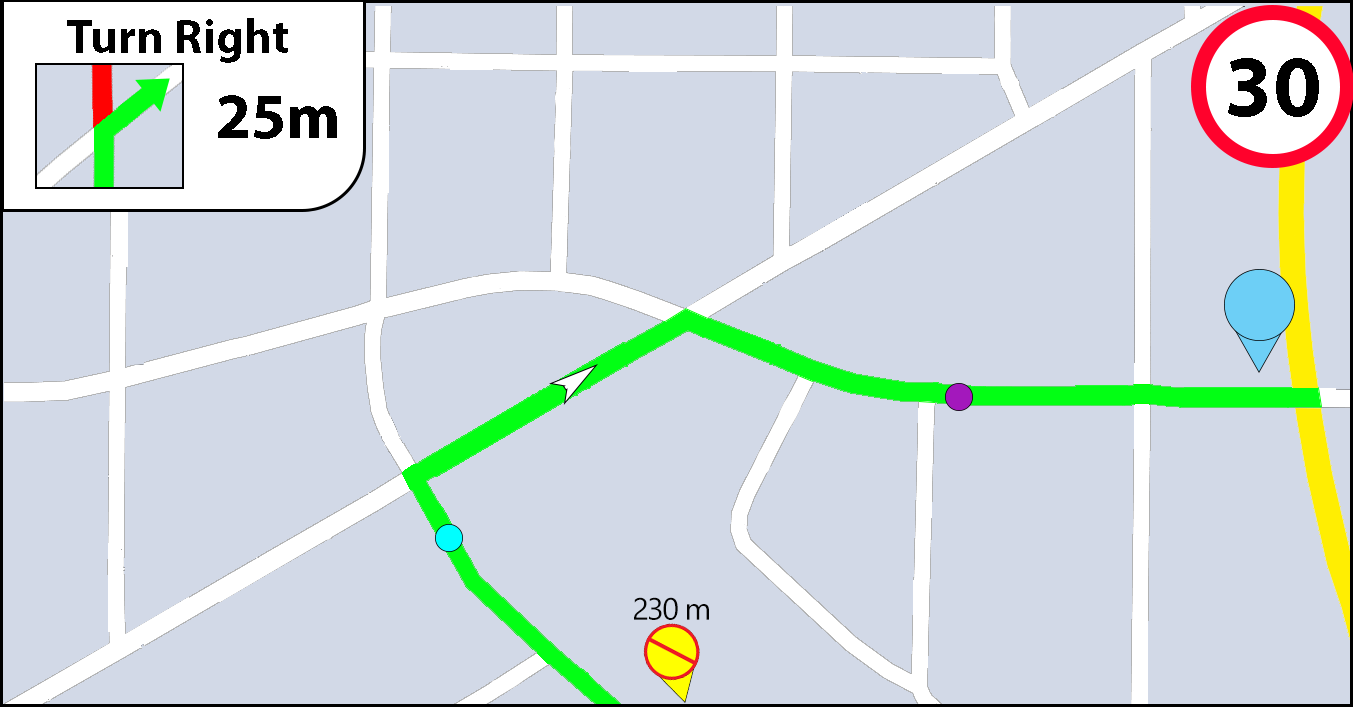
\includegraphics[scale=0.3]{convoy-map}
  \caption{Hi-Fi final design for navigation including convoy members. Please note that this design shows a static map, whereas the map in the final design will rotate to keep the user facing forward}\label{convoy-map}
\end{figure}
During navigation, this map design in Figure~\ref{convoy-map} represents what is shown on the dedicated navigation screen (only, with a rotating map). We created this design to show off a lot of features at the same time: an instruction window in the top left describes the movement to take, a distance, and a preview of the junction; the current speed limit is shown in the top right, for the current road the driver is on.

Furthermore, a lot of convoy features are shown here: there is a waypoint by the yellow road, signifying a place that the group has already agreed to stop and meet at; the yellow car is too far away to be shown on the map, so is shown at the edge of the map with an indication of how far away they are; and also, the yellow car has made an unplanned stop, so is overlaid with a red cross.

This prototype is expanded by means of an animation, which can be found at \url{http://imgur.com/a/xck0U}, which shows how the interface handles other cars losing connection; cars reaching an expected stop; and cars moving while still out of map range.

%\subsection{Final design}\label{ssec:nav-final-design}

\subsection{Evaluation}\label{ssec:nav-evaluation}


%%%%%%%%%%%%%%
%
%	APP
%
%%%%%%%%%%%%%%
\section{Feature 2: App}\label{sec:app}

\subsection{Research}\label{ssec:app-research}
Research and brainstorming were conducted in a cyclic manner to ensure that the latest technologies relevant to this sector of the automotive industry were taken into consideration. Extensive research revealed that most leading companies such as Jaguar [\cite{jaguar-ws}], BMW [\cite{bmw-ws}] and Tesla[\cite{tesla-ws}] already offer multi-platform mobile apps that compliment their automobiles. Each of the above boasts at least one of the features that we intended to integrate into our systems such as remote control and seamless route porting from smartphone to car. From brainstorming through to coding the prototype, our focus was directed on how to improve on existing products and also integrate our novel features.
The research methods we used included a questionnaire, installing and using manufacturers apps on our mobile devices, browsing their websites and reading through papers and articles found through numerous searches on search engines.

While browsing the existing apps that manufacturers offer, we have come across some flaws that  we were determined to get right in our final product. For example, \textit{BMW Connected}, their take on an app to compliment their most recent cars, excels in features like learning driving habits over time and facilitating safe communication with friends and family while still requiring a wired connection for simple features like transferring a route from the phone to the cars' navigation system and having a restricted range for remote functions such as lock, beep horn and switch lights. Flaws of similar magnitude con be found in \textit{Jaguar In-Control apps} and \textit{Mercedes Me}, which is reviewed as unusable or useless by most users.

We found that even where features are collectively good, they are often scattered over several apps, we intended for our customers to be able to download one app and be able to access all features from there while keeping it intuitive and user-friendly.

Part of the second iteration of research involved looking into how useful different types of people find different features. This was achieved by polling friends and family of each of us, and therefore diversifying ethnicity, background and locations. We have then attached each to each of our features discussed in the brainstorming session to some personas for whom it would be relevant and this helped us decide how to prioritise our ideas.

\subsection{Brainstorming}\label{ssec:app-brainstorming} % Chris
When brainstorming ideas for the accompanying app for our car system, we considered both functional and non-functional requirements. We opened up a Google Doc so that we would all be able to contribute and follow along quickly since we all knew we had a lot of ideas for app integration features. One of the reasons that we all had so many ideas already was because we had already suggested certain ideas while planning features for the car's system previously.

We didn't rule out any ideas at this stage since even the most ridiculous ideas can spark inspiration for a more realistic and useful idea (``no idea's a bad idea''). Not ruling out ideas also kept our brainstorming phase moving quickly and meant that people were happy to go ahead with anything they thought of.

Once we couldn't come up with any more ideas for our initial brainstorm, we grouped each idea by features in a separate ``refined ideas'' document one by one after first discussing whether the idea was feasible and worth expanding upon. Once we had our completed refined and grouped ideas document, we were ready to start designing and researching technical details.

A section of our initial ideas brainstorming document can be seen in Figure~\ref{initial-ideas} and a section of our refined ideas can be seen in Figure~\ref{refined-ideas}.

\begin{figure}[H]
  \centering
  \fbox{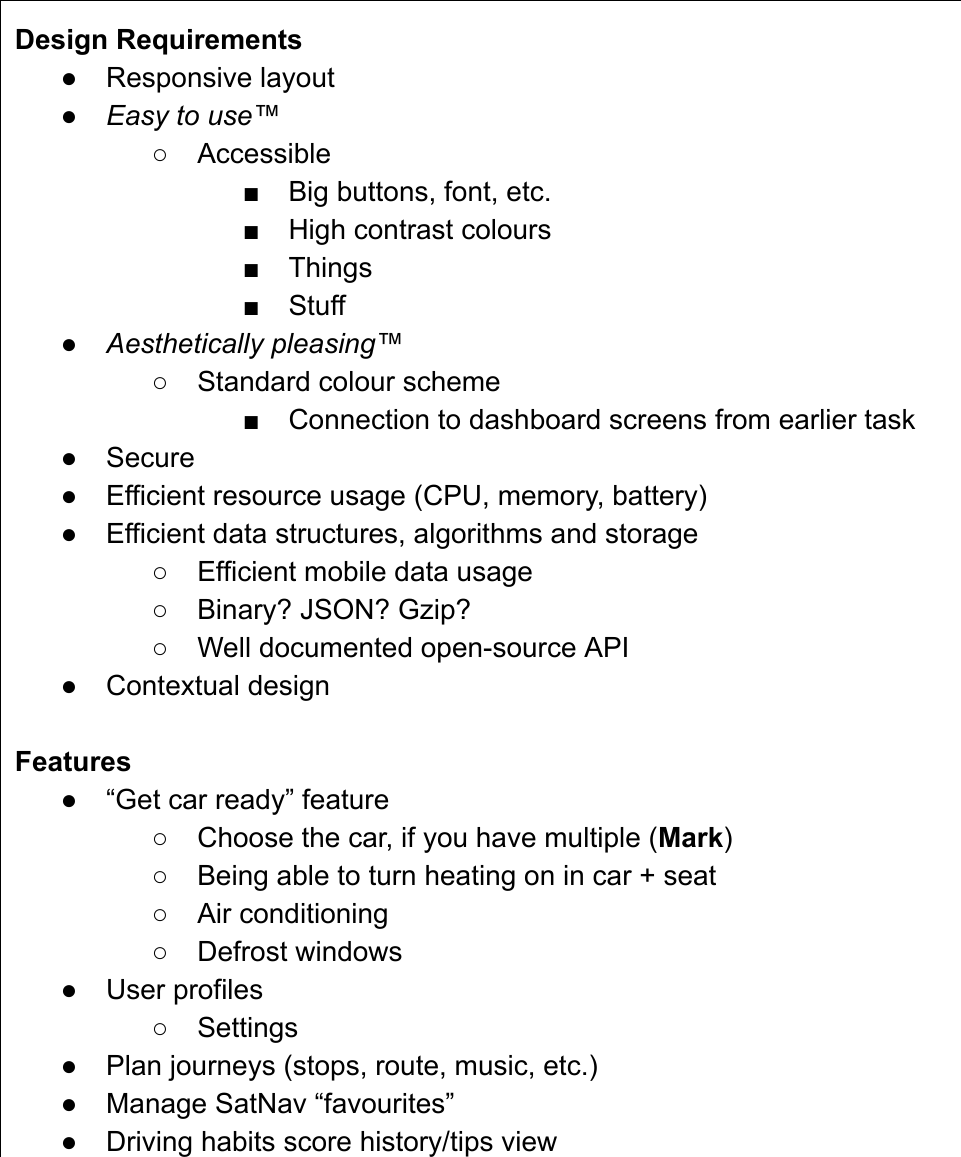
\includegraphics[scale=0.25]{initial-ideas}}
  \caption{Initial ideas brainstorming document.}\label{initial-ideas}
\end{figure}

\begin{figure}[H]
  \centering
  \fbox{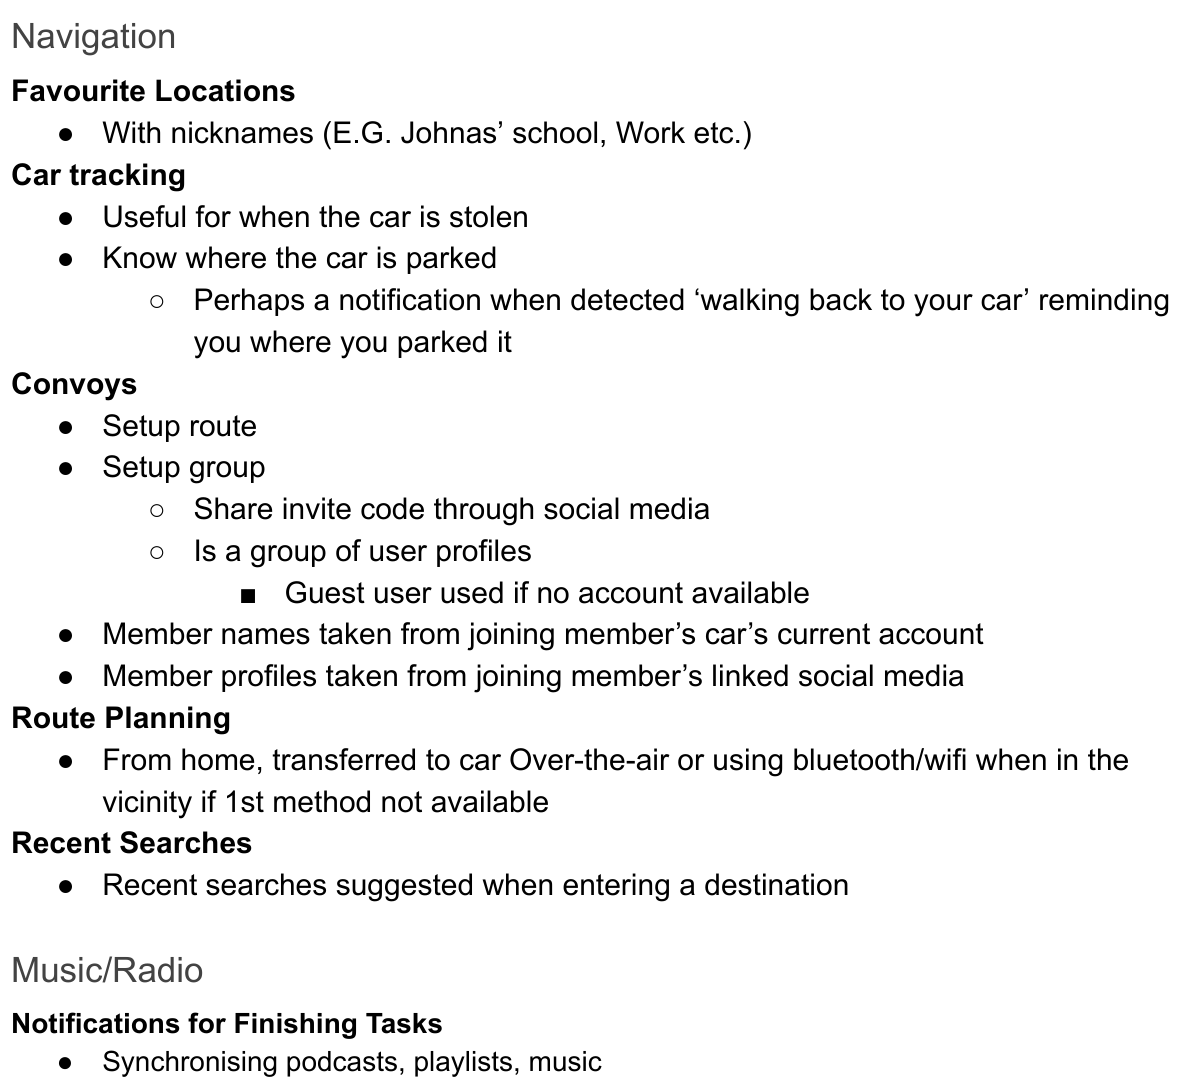
\includegraphics[scale=0.25]{refined-ideas}}
  \caption{Refined ideas document.}\label{refined-ideas}
\end{figure}

\subsection{Technical Background}\label{ssec:app-tech} % Tyler
Many features of the app rely on communication with the car in order for them to work. These messages are sent between the phone to the car's central computing unit to be processed. Features which send instructions to the car to control the car's hardware have two different types of communication.

Firstly, instructions such as turn the heating on or toggling headlights will be on an on/off basis. For example setting the temperature to 20 degrees will keep it at that until it has changed.

Secondly, instruction-critical tasks such as remote controlling the car with the phone app, rapidly send instructions to the car to ensure the car is performing actions safely and as the user expects. For example, if a user is holding the steering wheel at a 45-degree angle, the associated instruction will be sent constantly and processed by the central computing unit until the user changes the rotation. If the phone would happen to lose connection and the instructions stop being received by the car, the car is stopped.

Features for controlling music within the car are communicated over Wi-Fi and Bluetooth. The local music library of the car is synced with the phone, and also there is a Spotify account linked to the driver's user profile. Which is logged in on the centre console.

All messages regarding the control of music with the app, are encapsulated within a JSON object. These messages will hold instructions such as play, pause and song requests. Song requests will contain music file names and the library they are stored in.
If music is from Spotify, then associated actions for controlling the Spotify account, which is logged in on the centre console are embedded within the message.

There is also the option to control the centre console Spotify account using Spotify's ``Spotify Connect'' service. This allows you to control other Spotify devices on the same network. The Wi-Fi network of the car in this case.

Users can also view the car cameras live video feed on their phones through our app. This video stream will be dynamically re-encoded by the cars computing unit and then transmitted over RTSP (Real Time Streaming Protocol). This is to make the best use of the connection of the car by adjusting the bitrate of video based on the available bandwidth from the car and to the client, whether they are connected via Wi-Fi or slow mobile data.

The app shares a lot of the same data structures for maps and caching, see Section~\ref{ssec:data-structures}~[\nameref{ssec:data-structures}] for more details.

\subsection{Design choices \& argumentation}\label{ssec:app-design}


Our app is designed with a flat design. This aims to keep the interface minimalistic in the use of shading and colour gradients, keeping the elements looking flat against the background. Flat design is a standard in the mobile industry, so users are familiar with this design and it is proven to be a clear interface design.

The colour scheme in the app is synchronised with the colour schemes of the centre console and the rear door screens, but can be overridden in the settings. This also aims to keep the user feeling in a familiar environment when using any part of the car system.

\begin{figure}[H]
  \centering
  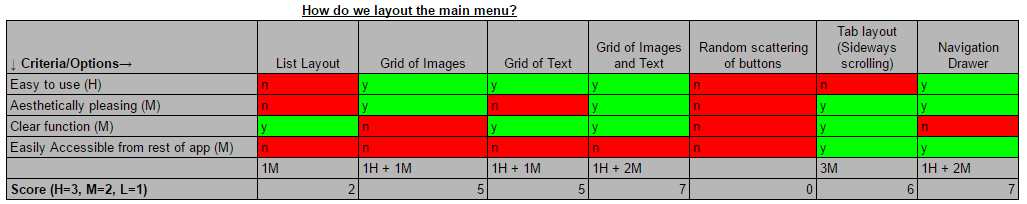
\includegraphics[scale=0.6]{qoc-app-menu}
  \caption{QOC discussing how to lay out the main menu}\label{qoc-app-menu}
\end{figure}

Figure~\ref{qoc-app-menu} asks how we can lay out the main menu. Since this is an aesthetic design choice, the criteria focus on ensuring ease of use and accessibility. As can be seen from the matrix, it is clear that there are multiple good options: grid of images and text, which adds clarity to possibly ambiguous images while making it more aesthetically pleasing than a grid of text; tabbed layout, which places all the features on the main screen and scrolls sideways between them; and a navigation drawer - a vertical bar accessible at the side of the screen offering links to the different features.

We decided to utilise all three of these options, which can be seen in Section~\ref{ssec:app-prototypes-testing}~[\nameref{ssec:app-prototypes-testing}], having a main menu with a grid layout of buttons showing image and text, which aims to mitigate the unclear functionality of a grid of only images through use of a textual description as well as using easily identifiable icons; a tab layout on the main menu to switch between a feed screen and the main menu; and a navigation drawer to allow easy access to a main menu from anywhere in the app.

\begin{figure}[H]
  \centering
  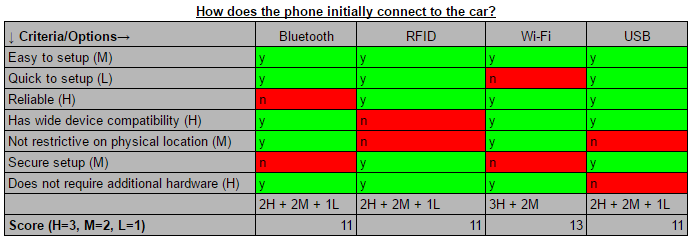
\includegraphics[scale=0.8]{qoc-app-connect}
  \caption{QOC discussing how to initially pair the car with the phone}\label{qoc-app-connect}
\end{figure}

Figure~\ref{qoc-app-connect} asks how the phone should initially connect to the car. These options are fairly close to each other in suitability, so we allow the user to use any of these methods for initial connection. However, after this initial connection, Wi-Fi is automatically paired so that the initial connection is no longer required, since this removes the restriction on the physical location of the device that RFID and USB suffer from (since both of these options require close proximity to a certain location in the car).

Initially, we had intended for RFID to be the method for primary connection to the car, since we thought it would be the easiest to use. However, the QOC showed us that having wide device compatibility is a really important criteria for this, which is not true of RFID.

\begin{figure}[H]
  \centering
  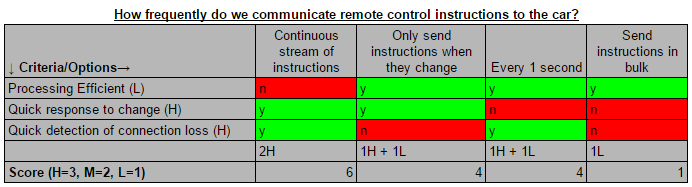
\includegraphics[scale=0.8]{qoc-app-remote}
  \caption{QOC discussing how frequently to send remote control instructions}\label{qoc-app-remote}
\end{figure}

Figure~\ref{qoc-app-remote} asks how frequently the phone should send instructions to the car while operating the remote control feature. Remote controlling a car is a task where safety must be of paramount as we are dealing with heavy machinery. Since remote control is heavy relied on communication we tried to decide on how fast we should be sending messages. As you can see despite continuous streams of instructions  not being the best choice for processing messages efficiency wise, it is quick for responding to changes and detecting if the phone has disconnected. This is more important so that is why we decided to go with continuous streams of instructions.

\subsection{Prototypes \& user testing}\label{ssec:app-prototypes-testing}
\begin{figure}[H]
  \centering
  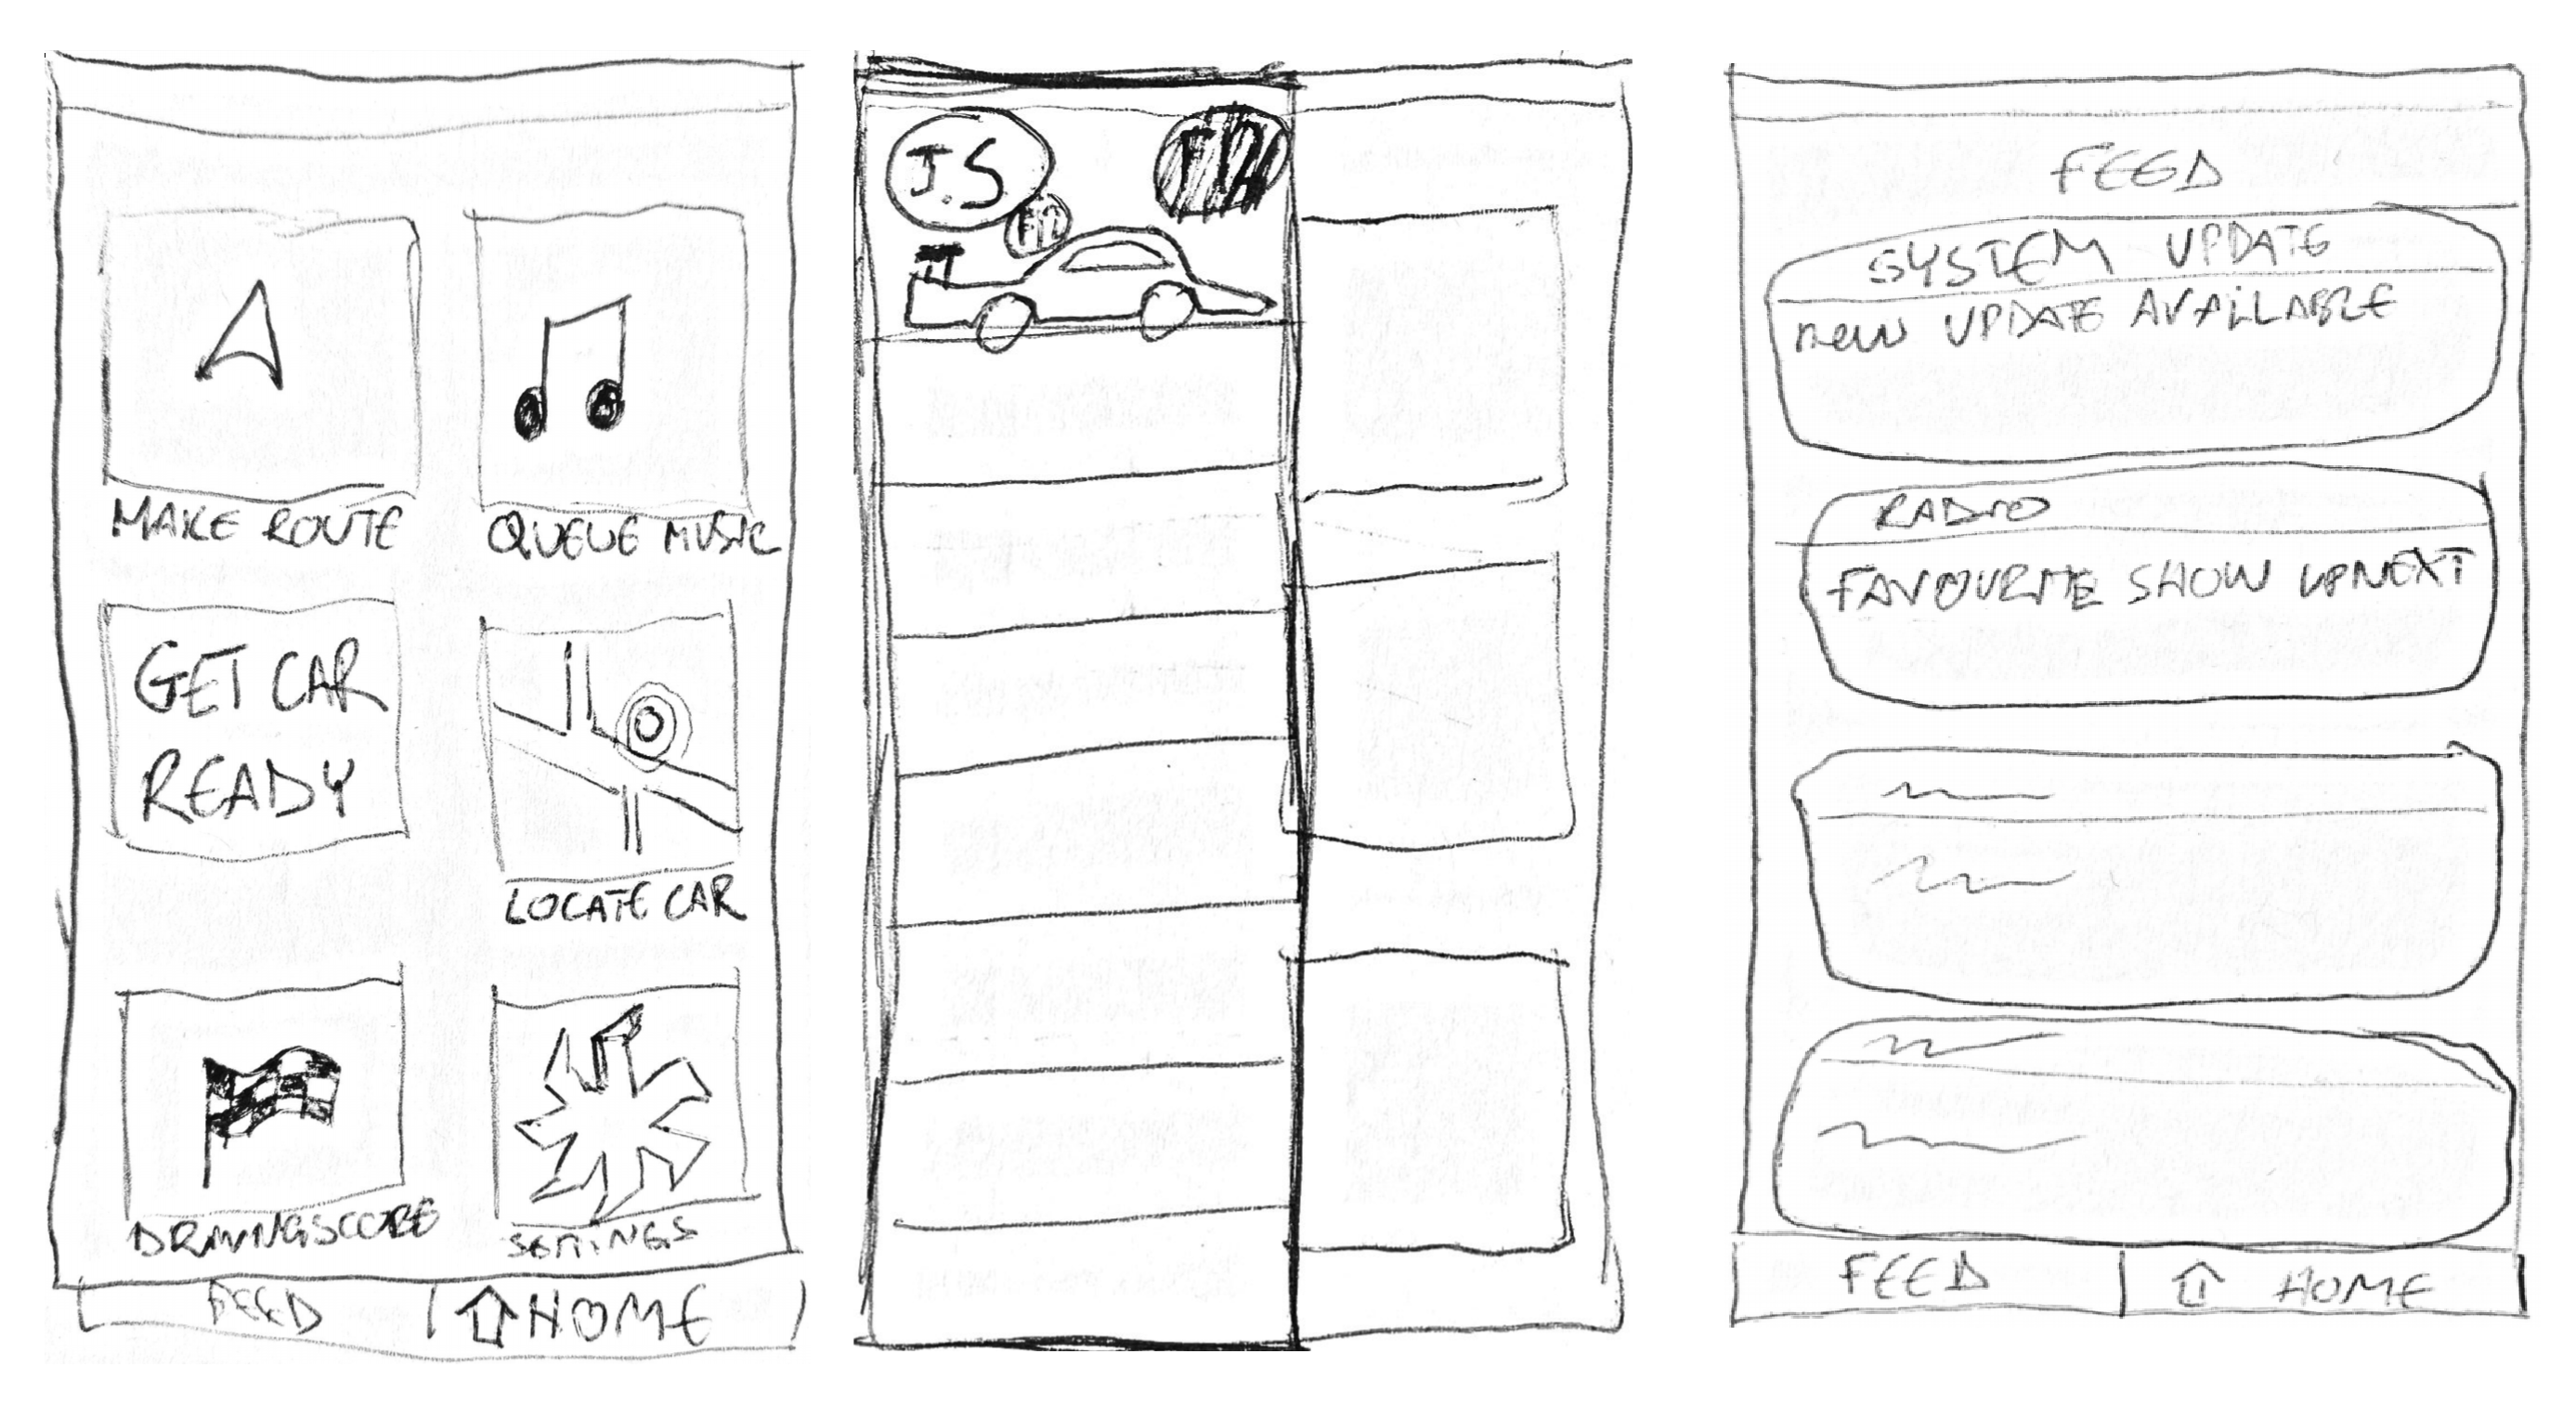
\includegraphics[width=\textwidth]{app-lofi}
  \caption{Lo-Fi prototypes of app interfaces}\label{figure-app-lofi}
\end{figure}

When designing a lo-fi prototype for the app's main screen, we already had a good idea of the features we would like to add to it. Mainly because we had pre-emptively thought there would be a task for designing an app. This made it easy to come up with a early design.

These designs follow the design choices we came to a conclusion to in the previous section. On the home screen interface (left most image of Figure \ref{figure-app-lofi}) we have large buttons paired with labels giving a brief description of what the buttons do. This provides an easy to use method for the users to go to any feature in the app, which is exactly what we wanted to achieve.

\begin{figure}[H]
  \centering
  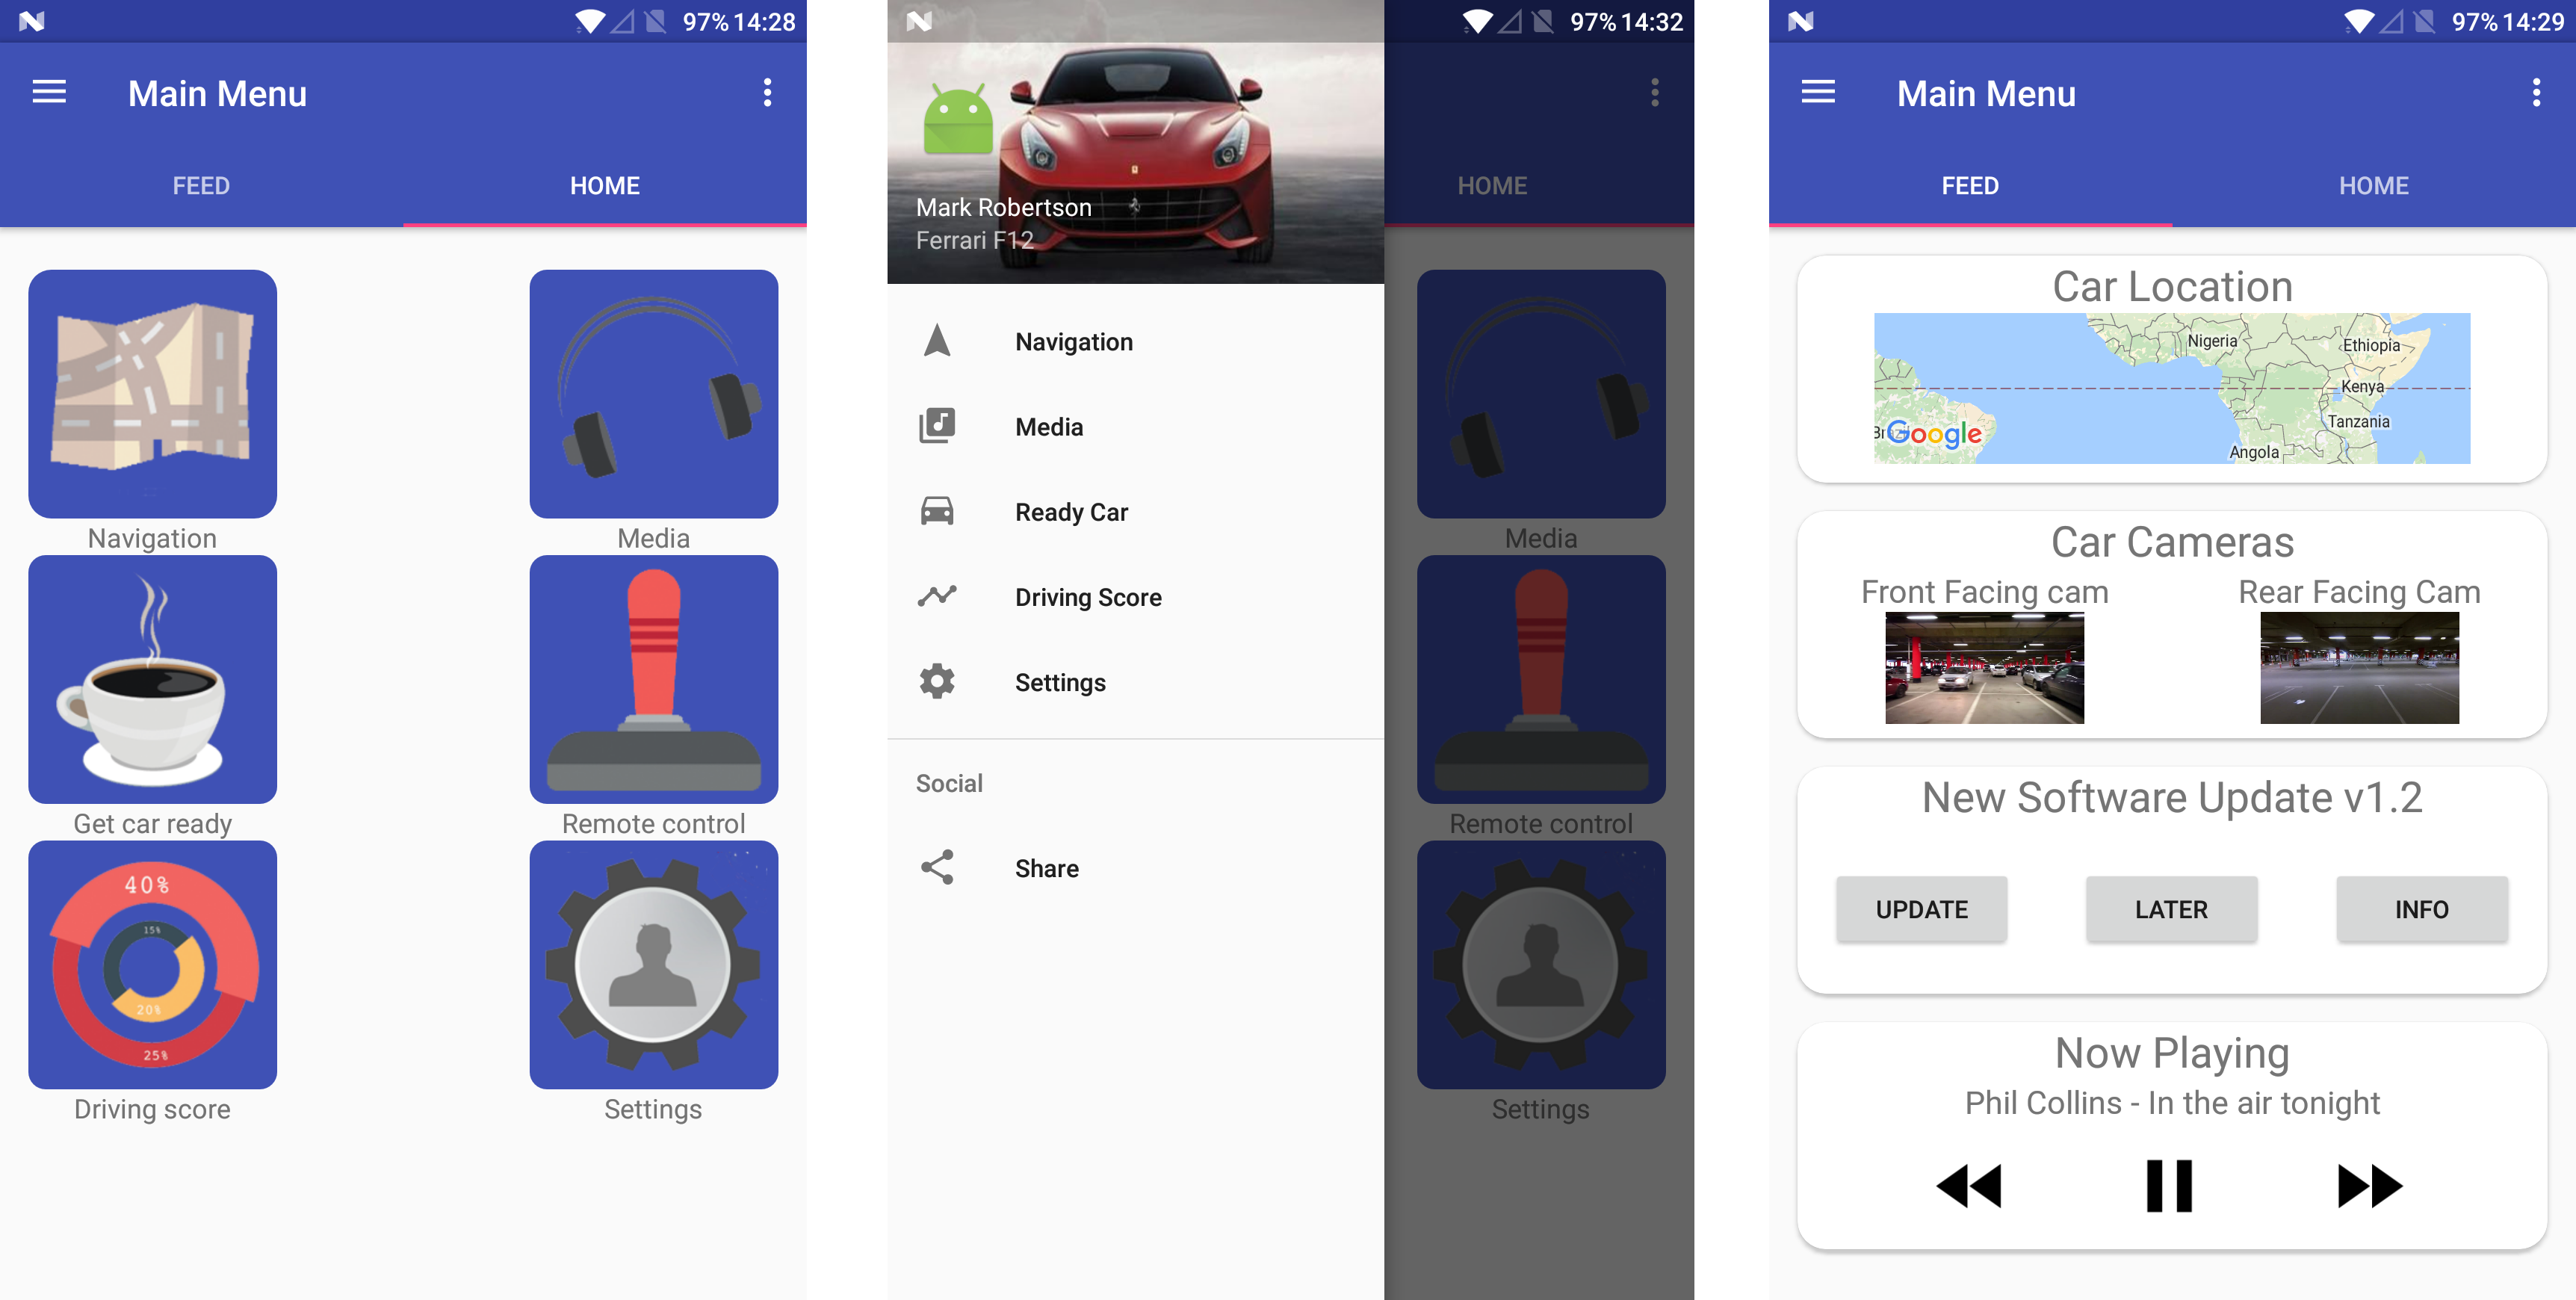
\includegraphics[width=\textwidth]{app-hifi}
  \caption{Hi-Fi prototypes of app interfaces.}\label{figure-app-hifi}
\end{figure}
Following our QOC decision we created a Hi-Fi version of our app interfaces which is our final design. This was built in Android Studio and the interfaces are navigable through the buttons on the navigation drawer.

The user can access the navigation drawer from any page within the app. This ensures ease of use and accessibility which is what we desired in our design choices.

On entering the app the user is prompted for to login or register an account. After successfully doing so they are presented with the feed interface (right most interface in Figure \ref{figure-app-hifi}) which is intended to show information based on the users context and latest updates. For example if users are away from their car they will have feed items such as car location and access to their car's cameras. This is because those features are intended to be used while the car owner is not with their car.

On the home screen (left most interface in Figure \ref{figure-app-hifi}) we have a simple list of functions, these are selectable buttons which have labels on them. This list is scrollable so more features can easily be added in the future. We successfully kept this design to follow the best QOC option that we found for laying out the main menu.

\subsection{App Security}\label{ssec:app-security}
On supported devices extra convenience methods for authenticating and unlocking app functionality will be provided to the users, extending all of the strong encryption and authentication methods that are put in place by the cloud and car systems.
\begin{itemize}
  \item Fingerprint unlocking: Using the built-in hardware store for safely keeping the user password, a fingerprint can be used on supported devices to release the password, instead of prompting the user to type it in when loading the app.
  \item Face recognition: Most commonly found on laptop computers with infrared cameras; this method of authentication isn't as secure as a biometric scanner as false-positive rates are typically higher however can identify and authenticate a user account in a similar way through the online portal or via a desktop app.
\end{itemize}

%\subsection{Final design}\label{ssec:app-final-design}

\subsection{Evaluation \& How it Fits The System}\label{ssec:app-evaluation}


% \end{multicols}

\printbibliography

\section{Appendix}\label{sec:appendix}
\subsection{Documents}\label{ssec:appendix-docs}

\subsection{Other areas of the design}\label{ssec:appendix-other}

% ALL ANNOTATED SLIDES
%\includepdf{slides-annotated}
% ANNOTATED AND FULL-SIZE SLIDES

%\includepdf[pages=1-5]{slides}
%\includepdf[pages=6]{slides-annotated}
%\includepdf[pages=7]{slides}
%\includepdf[pages=8]{slides-annotated}
%\includepdf[pages=9]{slides}
%\includepdf[pages=10]{slides-annotated}
%\includepdf[pages=11]{slides}
%\includepdf[pages=12]{slides-annotated}
%\includepdf[pages=13-19]{slides}
%\includepdf[pages=20]{slides-annotated}
%\includepdf[pages=21-23]{slides}
%\includepdf[pages=24]{slides-annotated}
%\includepdf[pages=25-32]{slides}
%\includepdf[pages=33]{slides-annotated}
%\includepdf[pages=35-35]{slides}
%\includepdf[pages=36]{slides-annotated}
%\includepdf[pages=37-52]{slides}
%\includepdf[pages=53]{slides-annotated}
%\includepdf[pages=54]{slides}
%\includepdf[pages=55]{slides-annotated}
%\includepdf[pages=56-57]{slides}
%\includepdf[pages=58]{slides-annotated}
%\includepdf[pages=59-61]{slides}
%\includepdf[pages=62-65]{slides-annotated}
%\includepdf[pages=66-68]{slides}
%\includepdf[pages=69]{slides-annotated}
%\includepdf[pages=70-71]{slides}
%\includepdf[pages=72]{slides-annotated}
%\includepdf[pages=73-74]{slides}
%\includepdf[pages=75]{slides-annotated}
%\includepdf[pages=76-78]{slides}
%\includepdf[pages=79]{slides-annotated}
%\includepdf[pages=80]{slides}
%\includepdf[pages=81]{slides-annotated}
%\includepdf[pages=82-83]{slides}

\end{document}

% vim: set tabstop=2 shiftwidth=2:
